\chapter{Four Formulations of the SEAS Problem}
\label{chap:44rmulations4SEAS}
Different approaches for solving the 2D antiplane shear problem are possible. First, four formulations of the SEAS problem are provided along with their analytic Jacobian matrices. Two of them are fully implicit and allow only implicit time integration methods whereas the two others allow for both explicit and implicit methods. This presentation is followed by a discussion about numerical and computational aspects of the four formulations with a major focus on the efficiency of the Newton iteration needed for solving implicit methods.

\section{First order formulations}
\label{sec:44mul4SEAS__1stOrderODE}
Three out of the four formulations are of first order, which means that at most the first time derivative of the physical quantities $S$ and $\psi$ appears. The first formulation in \autoref{ssec:444SEAS__1stOrderODE} can be solved explicitly and was the only originally available whereas the formulations in \autoref{ssec:444SEAS__extendedDAE} and \autoref{ssec:444SEAS__compactDAE} are purely implicit. All analytic Jacobian matrices in this section have been derived in the scope of this thesis.

\subsection{Formulation as a first order ODE}
\label{ssec:444SEAS__1stOrderODE}
\subsubsection{Problem}
The first approach to solve the SEAS problem is to formulate the system as a classical ODE. The solution vector contains the values for the slip and the state variable. At each timestep, the slip rate $V$ is calculated from the friction law $F$ with the bisection method and the time derivative of the state $\dot{\psi}$ can be directly calculated from the ageing law $G$, both in \autoref{eq:DAEFormulation2DSEAS}. The friction law is continuously differentiable and its Jacobian matrix with respect to $V$ in \autoref{eq:partial_df_dV} is invertible, with $i$ the index of each of the $n$ fault nodes. Therefore the implicit function theorem can be applied and states that a solution $V$ exists in $\mathbbm{R}^n$ where $V_i(S,\psi)$ is a continuously differentiable function. This approach was the only originally available implementation in {\ttfamily tandem}.

\begin{align}
	\label{eq:ODE_formulation_SEAS}
	x &= \begin{pmatrix}
		S \\ \psi
	\end{pmatrix} & \dot{x} &= \begin{pmatrix}
								  \dot{S} \\ \dot{\psi}
							   \end{pmatrix} = \begin{pmatrix}
												   V(S,\psi) \\ G(\psi, V)
											   \end{pmatrix} = \Gamma
\end{align} 

This formulation allows us to use many well-known and proven implicit and explicit numerical schemes. 

\subsubsection{Jacobian matrix}
\label{sssec:Jacobian_ODE}
For the ODE formulation in \autoref{eq:ODE_formulation_SEAS} it is not straightforward to calculate the Jacobian matrix because of the implicit evaluation of the slip rate $V$. At each fault node the right-hand side $\Gamma_i$ contains one component for each $V_i$ and $G_i$ and the solution vector $x_i$ one component for each $S_i$ and $\psi_i$. Therefore, four Jacobian matrices of size $\mathbbm{R}^{n\cross n}$ are needed to describe the system for each combination of the components in $\Gamma$ and $x$. They can be assembled to one general Jacobian matrix $\mathbf{J}_\Gamma$ of size $\mathbbm{R}^{2n\cross 2n}$ with four block matrices:
\begin{equation}
\label{eq:Jacobian_ODE_formulation}
\mathbf{J}_\Gamma(S,\psi,V)_{ij} = \begin{pmatrix} 
\pdv{V_i}{S_j} &
\pdv{V_i}{\psi_j} \\ 
\pdv{G_i(\psi,V)}{S_j} &
\pdv{G_i(\psi,V)}{\psi_j}  \end{pmatrix}
\end{equation}
In a first step, the partial derivatives of the slip rate $V$ will be calculated. The second part of the implicit function theorem provides an expression for the Jacobian matrices with respect to $S$ and $\psi$:
\begin{align}
\label{eq:partial_V_S}
\pdv{V_i}{S_j} &= -\left(\pdv{F}{V}\right)_{ik}^{-1}\pdv{F_k}{S_j} \\ 
\label{eq:partial_V_psi}
\pdv{V_i}{\psi_j} &= -\left(\pdv{F}{V}\right)_{ik}^{-1}\pdv{F_k}{\psi_j}
\end{align}
Two of the occurring matrices can be easily calculated from the analytic expression of the friction law in \autoref{eq:DAEFormulation2DSEAS}. A generalized Kronecker delta $\delta_{ij}^k$ is defined as 1 if $i=j=k$ and 0 otherwise.
\begin{align}
\pdv{F_i(S,\psi,V)}{\psi_j} &= \left( -\frac{\sigma_n}{2V_0} \frac{Ve^{\frac{\psi_k}{a}}}{\sqrt{\frac{e^{\frac{2\psi_k}{a}}V_k^2}{4V_0^2}+1}}\right)\delta_{ij}^k 
\label{eq:partial_df_dpsi} \\
\pdv{F_i(S,\psi,V)}{V_j} &= \left( -\frac{a\sigma_n}{2V_0} \frac{e^{\frac{\psi_k}{a}}}{\sqrt{\frac{e^{\frac{2\psi_k}{a}}V_k^2}{4V_0^2}+1}}-\eta\right)\delta_{ij}^k 
\label{eq:partial_df_dV}
\end{align}
Since $\pdv{F}{V}$ is a diagonal matrix, its inverse is very easy to calculate and does not require us to solve a linear system of equations. \\
The third derivative $\pdv{F}{S}$ is more complicated to obtain. In the friction law, $S$ appears only in the expression of the traction term $\tau$, so $\pdv{F}{S}=\dv{\tau}{S}$. As shown in \autoref{apx:dtau_dS}, it is a constant dense matrix. To precompute it, the computationally expensive DG problem needs to be solved $n$ times, where $n$ is the number of fault nodes. \\

To express the full Jacobian matrix of the ODE in \autoref{eq:Jacobian_ODE_formulation}, the partial derivatives of the ageing law $G$ are also required. They can be expressed in term of the already known partial derivatives: 
\begin{align}
	\pdv{G_i}{S_j}    &= -\frac{b}{L}\pdv{V_i}{S_j} \\
	\pdv{G_i}{\psi_j} &= -\frac{V_0}{L}e^{\frac{f_0 - \psi_k}{b}}\delta_{ij}^k -
						  \frac{b}{L}\pdv{V_i}{\psi_j}
\end{align}



\subsection{Formulation as a DAE}
\label{ssec:444SEAS__extendedDAE}
\subsubsection{Problem}
The ODE form may not be ideal because of the implicit evaluation of the slip rate, which is treated independently of the numerical integration. Alternatively, the friction law could be solved for the slip rate together with $S$ and $\psi$. The solution vector is then extended by one quantity and $V$ is not evaluated with a separate iterative scheme anymore.
\begin{align}
	\label{eq:DAE_formulation_SEAS}
	x &= \begin{pmatrix}
			S \\ \psi \\ V
		 \end{pmatrix} & \dot{x} &= \begin{pmatrix}
										\dot{S} \\ \dot{\psi} \\ 0
									\end{pmatrix} = \begin{pmatrix}
										V \\ G(\psi, V) \\ F(S,\psi,V)
									\end{pmatrix}
\end{align}
This formulation necessarily requires an implicit time integration method which iteratively solves for the time-variant quantities $S$ and $\psi$ as well for the algebraic state $V$. The main difference to the ODE formulation with an implicit method is the sparser structure of the Jacobian matrix. The arising linear system can be solved more efficiently with direct and iterative solvers as it will be discussed in detail in \autoref{ssec:iterative_solver_Jacobian}. \\
The PETSc interface requires us to provide a DAE in the form
\begin{align}
	\Phi(t, x,\dot{x}) = \Gamma(t,x) 
\end{align}
where the left-hand side function $\Phi$ depends on the solution vector and its time derivative whereas the right-hand side function $\Gamma$ only depends on the solution vector. For now, we choose a fully implicit formulation of the problem, in which $\Gamma$ vanishes. The DAE can then be expressed in the following way: 
\begin{align}
\label{eq:DAE_extended_formulation_SEAS}
	x &= \begin{pmatrix}
		S \\ \psi \\ V
	\end{pmatrix} & \Phi(t, x,\dot{x}) &= \begin{pmatrix}
	 	V - \dot{S} \\ G(\psi, V) - \dot{\psi}  \\ F(S,\psi,V)
	\end{pmatrix} = \begin{pmatrix}
		0 \\ 0 \\ 0
	\end{pmatrix} = \Gamma(t,x)
\end{align}

Another class of solvers, the so-called IMEX (implicit-explicit) solvers \cite{IMEX}, offer an interesting approach to numerically solve this problem, by mixing an implicit, iterative method for the algebraic states with an explicit method for the remaining simple time-dependent quantities. Technically, the function $\Phi$ is expected to be integrated implicitly, while the right-hand side function $\Gamma$ is solved explicitly. In the given formulation, we could shift the time derivatives of $S$ and $\psi$ to the right-hand side of the equation. This approach is not further considered in this thesis, but might be worth looking at in future work.

\subsubsection{Jacobian matrix}
\label{sssec:Jacobian_DAE}
For the DAE formulation of the system in \autoref{eq:DAE_extended_formulation_SEAS}, another approach can be chosen to calculate the Jacobian matrix of the system. With now three different components in the solution vector, the Jacobian matrix contains the partial derivatives with respect to the slip rate in addition to the slip and to the state variable. Similarly, the function $\Phi$ on which the Jacobian is applied is extended by the friction law. Each block $(i,j)$ in the structure of the Jacobian is given by:
\begin{equation}
\label{eq:Jacobian_DAE_formulation}
\mathbf{J}_\Phi(S,\psi,V)_{ij} = \begin{pmatrix}
\pdv{V_i}{S_j} & \pdv{V_i}{\psi_j} & \pdv{V_i}{V_j} \\
\pdv{G_i(\psi,V)}{S_j} & \pdv{G_i(\psi,V)}{\psi_j} & \pdv{G_i(\psi,V)}{V_j} \\
\pdv{F_i(S,\psi,V)}{S_j} & \pdv{F_i(S,\psi,V)}{\psi_j} & \pdv{F_i(S,\psi,V)}{V_j}
\end{pmatrix}
\end{equation}
In the previous section, a complicated approach had to be followed to obtain the derivative for the slip rate because of the nonlinear friction law, which was indirectly solved for each evaluation of the slip rate. Since the slip rate is now obtained directly from the solution vector $x$ and not from an iterative solver for the friction law, all its partial derivatives except with each component itself vanish. 

\begin{align}	
\pdv{V_i}{S_j} &= 0 & \pdv{V_i}{\psi_j} &= 0 & \pdv{V_i}{V_j} &= \delta_{ij}
\end{align}

Similarly, the partial derivatives of the ageing law can be directly evaluated from its definition in \autoref{eq:DAEFormulation2DSEAS}.
\begin{align}
\pdv{G_i(\psi,V)}{S_j} &=  0 &
\pdv{G_i(\psi,V)}{\psi_j} &= -\frac{V_0}{L}e^{\frac{f_0-\psi_k}{b}}\delta_{ij}^k &	
\pdv{G_i(\psi,V)}{V_j} &= -\frac{b}{L} \delta_{ij}
\end{align}
For the friction law, the Jacobian matrices have already been calculated in \autoref{eq:partial_df_dpsi} for $\pdv{F(S,\psi,V)}{\psi}$, in \autoref{eq:partialDerivative_df_dS} for $\pdv{F(S,\psi,V)}{S}$ and in \autoref{eq:partial_df_dV} for $\pdv{F(S,\psi,V)}{V}$.

This formulation of the Jacobian cannot be directly used in the Newton iteration to calculate the next timestep. Typically, the Jacobian has to be adapted to represent the time-stepping scheme. For instance, the implicit Euler method results requires to solve the nonlinear equation $0 = 1/h(x_n - x_{n+1}) + F(x_{n+1})$ for the solution at the next timestep $x_{n+1}$ and the Jacobian matrix $J_N$ for the corresponding Newton iteration is constructed from $J$. 
\begin{equation}
J_N = -\frac{1}{h}I + J
\end{equation}
Here, the problem arises that the time evolution is only defined for two components in the solution vector: the slip $S$ and the state variable $\psi$. The slip rate $V$ needs to be solved algebraically at every Newton iteration, but this component should not be included in the time-stepping scheme. The nonlinear equation to calculate a step of the implicit Euler has to be adapted to include properly the slip rate. 
\begin{align}
0 = \begin{pmatrix} \frac{1}{h}S_n     \\ \frac{1}{h}\psi_n     \\ 0 \end{pmatrix} - 
\begin{pmatrix} \frac{1}{h}S_{n+1} \\ \frac{1}{h}\psi_{n+1} \\ 0 \end{pmatrix} + 
\begin{pmatrix} V_{n+1}            \\ g(\psi_{n+1},V_{n+1}) \\ f(S_{n+1}, \psi_{n+1}, V_{n+1}) \end{pmatrix}
\end{align}
The Jacobian matrix to be used in a Newton iteration to solve this problem has to be changed accordingly.
\begin{align}
\label{eq:Jacobian_Newton_Iteration_extended_DAE}
\mathbf{J}_N = 
\begin{pmatrix} 
-\frac{1}{h}\mathbf{I} & \mathbf{0}            & \mathbf{0} \\ 
\mathbf{0}             &-\frac{1}{h}\mathbf{I} & \mathbf{0} \\ 
\mathbf{0}             & \mathbf{0}            & \mathbf{0} 
\end{pmatrix} + 
\begin{pmatrix}  
\mathbf{J}_S(S)    &  \mathbf{J}_\psi(S)    &  \mathbf{J}_V(S)    \\ 
\mathbf{J}_S(\psi) &  \mathbf{J}_\psi(\psi) &  \mathbf{J}_V(\psi) \\ 
\mathbf{J}_S(V)    &  \mathbf{J}_\psi(V)    &  \mathbf{J}_V(V)
\end{pmatrix} =
\begin{pmatrix} 
-\frac{1}{h}\mathbf{I}         &  \mathbf{0} 			            &
\mathbf{I}                     \\ 
\mathbf{0}                    & 
-\frac{1}{h}\mathbf{I} +  \pdv{g}{\psi}       &  \pdv{g}{V} \\ 
\pdv{f}{S} & \pdv{f}{\psi} &  \pdv{f}{V} 
\end{pmatrix}
\end{align}
If other implicit numerical schemes are used than the implicit Euler, such as higher-order BDF methods, $\mathbf{J}_N$ can be easily changed by multiplying the identity matrices $\mathbf{I}$ with a coefficient that depends on the chosen method. Albeit this formulation of the Jacobian matrix is perfectly valid, it is very specific to the SEAS problem and is therefore hard to implement as such within the PETSc framework. \\
To solve general implicit DAEs of the form $\Phi(t,x,\dot{x}) = \Gamma(t,x)$, PETSc offers a convenient interface to provide the Jacobian matrices. In fact, three matrices have to be provided. The first Jacobian matrix, denoted by $\bm{\Gamma}_{\dot{x}}$, corresponds to the variation of the left-hand side function $\Phi$ with respect to the derivative of the solution vector. The second matrix $\bm{\Gamma}_x$ describes the variation of the same function under the actual solution vector. Finally, the third Jacobian matrix $\bm{\Gamma}_x$ represents the variation of the right-hand side function $\Gamma$ under the influence of $x$. In our case, the formulation is fully explicit and the right hand side function $\Gamma(t,x)$ is zero everywhere, and by extension, its Jacobian matrix $\bm{\Gamma}_x$ also vanishes. It remains to express the Jacobian matrix of the Newton iteration $\mathbf{J}_N$ in terms of $\bm{\Phi}_x$ and $\bm{\Phi}_{\dot{x}}$:
\begin{equation}
\mathbf{J}_N = \frac{d\Phi}{dx_n} = \bm{\Phi}_{\dot{x}}\frac{d\dot{x}_n}{dx_n} + \bm{\Phi}_x	
\end{equation}
The term $\frac{d\dot{x}_n}{dx_n}$ is a scalar and depends only on the chosen timestep scheme, which can be denoted by $\sigma$. For the implicit Euler method for instance, we have $\sigma = 1/h$. The Jacobian matrix $\bm{\Phi}_x$ is exactly the one expressed in \autoref{eq:Jacobian_DAE_formulation} and $\bm{\Phi}_x$ contains negative identity matrices at the entries for the slip $S$ and for the state variable $\psi$.
\begin{align}
\bm{\Phi}_x = \begin{pmatrix} 
\mathbf{0}                     &  \mathbf{0}                       & 
\mathbf{I}                    \\ 
\mathbf{0}                     &  \pdv{G}{\psi} & 
\pdv{G}{V} \\ 
\pdv{F}{S}  &  \pdv{F}{\psi} &  
\pdv{F}{V} 
\end{pmatrix} &&&
\bm{\Phi}_{\dot{x}} = \begin{pmatrix} 
-\mathbf{I}  &  \mathbf{0}  & \mathbf{0} \\ 
\mathbf{0}  & -\mathbf{I}  & \mathbf{0} \\ 
\mathbf{0}  &  \mathbf{0}  & \mathbf{0}
\end{pmatrix}
\end{align}
With these two matrices, the Jacobian matrix for the Newton iteration of the implicit Euler method is the same as calculated in \autoref{eq:Jacobian_Newton_Iteration_extended_DAE}.



\subsection{Compact formulation as a DAE}
\label{ssec:444SEAS__compactDAE}
\subsubsection{Problem}
It is important to remember that the slip rate is the time derivative of the slip, so the variables $\dot{S}$ and $V$ are equal and can be interchanged in the problem formulation. As such, the friction law can be solved directly for $\dot{S}$ and the term $V$ is not required anymore. The solution vector then remains with the components of the slip $S$ and of the state variable $\psi$, as previously in the ODE formulation.
 \begin{align}
	\label{eq:DAE_compact_formulation_SEAS}
	x &= \begin{pmatrix}
			S \\ \psi
	     \end{pmatrix} & \Phi(t, x,\dot{x}) &= \begin{pmatrix}
												F(S,\psi,\dot{S}) \\ G(\psi, \dot{S}) - \dot{\psi}
											\end{pmatrix} = \begin{pmatrix}
																0 \\ 0
															\end{pmatrix} = \Gamma(t,x)
\end{align}
As in the previous DAE formulation, the friction law is solved along with time-variant quantities $S$ and $\psi$. Therefore it can be only used with an implicit integrator. \\

\subsubsection{Jacobian matrix}
The compact DAE formulation of the problem in \autoref{eq:DAE_compact_formulation_SEAS} also requires to be solved fully implicitly and involves again the three Jacobian matrices, $\mathbf{F}_{\dot{x}}$, $\mathbf{F}_x$ and $\mathbf{G}_x$, where the last one also vanishes because the right-hand side function is zero. The block matrices that appear in this formulation are calculated in the same way as previously but are arranged differently.
\begin{align}
	\label{eq:Jacobian_compact_DAE}
	\bm{\Phi}_{\dot{x}}&=  \begin{pmatrix}
								\pdv{F}{V} &  \mathbf{0} \\
							    \pdv{G}{V} & -\mathbf{I}
							\end{pmatrix} & 
	\bm{\Phi}_x        &=  \begin{pmatrix}
								\pdv{F}{S} & \pdv{F}{\psi} \\
								\mathbf{0} & \pdv{G}{\psi}
							\end{pmatrix} & 
	\bm{\Gamma}_x        &=  \begin{pmatrix}
								\mathbf{0} & \mathbf{0} \\
							    \mathbf{0} & \mathbf{0}
							\end{pmatrix}
\end{align}

\subsection{Verification of the Jacobian matrices}
All Jacobian matrices defined in this section have been checked for correctness. For that, a second order central finite difference approximation \cite[p. 184]{introductionPartialDiffEquations} is used to approximate each term of the Jacobian. 
\begin{equation}
	\mathbf{J}_{ij} = \pdv{\Phi_i}{x_j} \approx \frac{\Phi_i(x + he_j) - \Phi_i(x - he_j)}{2h}
\end{equation}
The function $F$ has to be evaluated $2n$ times with the current solution vector $x$ and a variation $h$ applied in positive and negative direction to each component of $x$ respectively. For this, the function to evaluate the right-hand side of the ODE or respectively the left-hand side for the DAEs is called. For an appropriate choice of $h$, not too large to be accurate and not too small to avoid truncation errors, the relative error between the analytic expression of the Jacobian and its approximation is inferior to $10^{-5}$ in all components and therefore, the expressions for the Jacobian matrices can be considered to be correct.

\subsection{Practical limitations of the Jacobian matrices}
The main advantage of implicit methods over explicit methods is to allow larger timesteps without accuracy loss. The program execution is therewith expected to be accelerated. The proposed calculation of the Jacobian matrix and its application in Newton iterations comes along with some drawbacks concerning the required calculation effort. \\
As described in \autoref{sssec:Jacobian_ODE}, the computation of the Jacobian matrix can be split up in one constant part $\pdv{\tau}{S}$ that has to be evaluated once at the beginning of the simulation and only depends on the domain geometry and in one variable part, that needs to be updated after each evaluation of the solution vector $x_n$. The initialization can be quite computationally expensive, as it requires, for each column of $\pdv{\tau}{S}$, to solve the Discontinuous Galerkin system for the entire domain with the corresponding unit vector as right-hand side vector. Each calculation of this linear system is approximately as expensive as performing one timestep with an explicit solver, since solving the same linear system is the most expensive operation of a timestep. For large domains with several hundred or thousand fault elements, which each contains a couple of fault nodes, this initialization operation takes a considerable amount of time. In comparison with an explicit scheme, a potential implicit method starts the race for the fastest solver with a penalty of about $n$ explicit timesteps, where $n$ is the total number of nodes on the fault. The advantages of implicit methods will therefore only pay off after a high number of iterations and make such methods of interest only if the simulated time frame is very long. This is typically the case because current simulations of sequences of earthquakes over several centuries with a high mesh resolution require up to a million timesteps with explicit methods. \\
Another potential drawback of the Newton method is that a linear system of size $n$ needs to be solved at each iteration step. This might still sound much less than solving for the displacement on the whole DG-domain of size $N$ as it is required to evaluate the right-hand side of the ODE at each iteration too. However, the DG system has a constant matrix $A$ whose LU-decomposition can be calculated once at the beginning of the simulation and each evaluation of the right-hand side only requires a backward substitution of complexity $\mathcal{O}\left(N^2\right)$. For the Jacobi matrix, such a pre-processing is not available since it changes along with the solution vector. Every calculation to solve the linear system in the Newton iteration is achieved with a complexity of the order $\mathcal{O}\left(n^3\right)$. In particular in large domains with many fault nodes, the solver with cubic complexity involves a substantially higher execution time than the one with quadratic complexity. 

\subsection{Iterative solvers for the Jacobian matrices}
\label{ssec:iterative_solver_Jacobian}
As discussed in the previous section, a linear system of equations has to be solved at each Newton iteration, and since the Jacobian matrices depend on the current solution vector, an expensive LU decomposition in $\mathcal{O}\left(n^3\right)$ has to be calculated at each step. This can be avoided with iterative solvers, which reduce the complexity of each Newton step to $\mathcal{O}\left(kn^2\right)$, where $k$ is the number of iterations in the matrix solver. \\
For the two DAE formulations, the partial sparse structure of the Jacobian matrix can be used to reformulate the system of equations in a way that iterative methods can be applied efficiently. We use the fact that among all submatrices, that are used to set up the Jacobian matrix, the only dense matrix is the constant term $\pdv{f}{S}$, and all other terms, are diagonal matrices. Let us consider the example of the Jacobian of the compact DAE formulation in \autoref{eq:Jacobian_compact_DAE}, with the linear system in which it appears in the Newton iteration. The dense term is denoted by the matrix $\mathbf{B}$ and all other block matrices $J_{ij}$ are diagonal.
\begin{equation}
	\begin{pmatrix}
		\mathbf{B} & \mathbf{J}_{12} \\ 
		\mathbf{J}_{21} & \mathbf{J}_{22} 
	\end{pmatrix} \begin{pmatrix}
		x_1 \\ x_2
	\end{pmatrix} = \begin{pmatrix}
		b_1 \\ b_2
	\end{pmatrix} 
\end{equation}
The vector $x$ describes the change in each component at the current Newton step and is the searched unknown and $b$ contains the left-hand side of the DAE system. Under the assumption that there are no zero entries on the diagonals, we first transform the Jacobian matrix to a lower triangular block matrix and obtain the following modified system: 
\begin{equation}
	\begin{pmatrix}
		\mathbf{B} - \mathbf{J}_{12}\mathbf{J}_{22}^{-1}\mathbf{J}_{21} & \mathbf{0} \\ 
		\mathbf{J}_{12} & \mathbf{J}_{22} 
	\end{pmatrix} \begin{pmatrix}
		x_1 \\ x_2
	\end{pmatrix} = \begin{pmatrix}
		b_1 - \mathbf{J}_{12}\mathbf{J}_{22}^{-1}b_2 \\ b_2
	\end{pmatrix} 
\end{equation}

Now, an iterative solver can be applied on the subsystem in the first line on the dense, but diagonally dominant to solve for the components in $x_1$. The components in $x_2$ can then be easily derived in $\mathcal{O}(n)$ operations with a forward substitution because all matrices $J_{ij}$ are diagonal. \\
A similar transformation was also obtained for the extended DAE formulation in \autoref{apx:ReducedJacobianExtendedDAE}, where the iterative solver is only required on a subsystem of size $n$ and where the missing components can be updated linearly in time. Without the reduction, no iterative methods with fast convergence could be found. For the first order ODE formulation, such a Gaussian elimination is not expedient because two out of the four submatrices are dense. However, iterative methods can directly be used on the entire Jacobian matrix.


\section{Second Order Differential Equation}
\label{sec:44mul4SEAS__2ndOrderODE}

So far, the original problem in \autoref{eq:DAEFormulation2DSEAS} has been formulated as a first order ODE in \autoref{eq:ODE_formulation_SEAS}, in which the friction law is solved implicitly within each evaluation of the right-hand side, such that explicit time integrators can be used. The solution vector has a compact size and only includes the slip $S$ and the state variable $\psi$. Alternatively, the problem can be directly formulated as a DAE, where the solution vector is extended by the slip rate $V$, such that it can be solved through the friction law iteratively together with the time quantities $S$ and $\psi$. A compact form of the DAE has also been formulated, where the derivative slip rate is directly used in the friction law instead of introducing a new variable~$V$. \\
The original motivation was to define an extended ODE formulation as counterpart to the extended DAE form, such that the solution vector contains an additional component for the slip rate $V$. To achieve this goal, it is necessary to find a function $H(t,S,\psi,V)$ which describes the change in time of the slip rate $\frac{dV}{dt}$. Since $V$ itself is the time derivative of the slip, this function $H$ corresponds to the second time derivative of the slip, or the slip acceleration. The new ODE formulation is: 
\begin{align}
&&	 x      =& \begin{pmatrix}	S                     \\ \psi           \end{pmatrix}      &
	 		   \begin{pmatrix}	\ddot{S}              \\ \dot{\psi}     \end{pmatrix}
			=& \begin{pmatrix}	H(t,S,\psi,\dot{S})   \\ G(\psi, V)     \end{pmatrix}
			 	 		 \\ &\Leftrightarrow&	 		  		 
	 x      =& \begin{pmatrix}	S       \\ \psi       \\ V	            \end{pmatrix}      &
   	\dot{x}  = \begin{pmatrix}	\dot{S} \\ \dot{\psi} \\ \dot{V}        \end{pmatrix}
	 		=& \begin{pmatrix}	 V      \\ G(\psi, V) \\ H(t,S,\psi,V)  \end{pmatrix}
	 		 = \Gamma	
	\label{eq:2nd_order_ODE_formulation}
\end{align}
Here, the friction law does not appear in the right-hand side anymore and is included in the function $H$. Unlike the previous ODE formulation, it does not require to solve the friction law implicitly at every timestep for the slip rate $V$ (or for any other quantity), therefore the new formulation is not a DAE anymore. Another beneficial advantage is, that if the boundary conditions of the DG domain are linear in time, it does not require solving the DG system at every timestep, which is the main performance bottleneck after initialization in the first order formulations. 

\subsection{Obtaining the second order ODE formulation}
This section will focus on the derivation of the right-hand side term $H(t,S,\psi,V)$, which is necessary to formulate the second order ODE. Starting point is the expression for the friction law in \autoref{eq:DAEFormulation2DSEAS}. At any time in the simulation, this algebraic equation always evaluates to zero, and therefore, its time derivative also vanishes. With the help of the formula of total derivatives, we obtain the following expansion: 
\begin{align}
	0 = \dv{F}{t} &= \pdv{F}{t} + \pdv{F}{S}\dv{S}{t} + \pdv{F}{\psi}\dv{\psi}{t} +  \pdv{F}{V}\dv{V}{t} \nonumber\\
					  &= \pdv{F}{t} + \pdv{F}{S}V + \pdv{F}{\psi}G(\psi,V) + \pdv{F}{V}H(t,S,\psi,V)
\end{align}
The partial derivatives of $F$ that occur are calculated in the same way as for the Jacobian matrices of the first order formulations. The terms $\pdv{F}{\psi}$ and $\pdv{F}{V}$ are diagonal matrices with the entries stated in \autoref{eq:partial_df_dpsi} and \autoref{eq:partial_df_dV} and the term $\pdv{F}{S}$ is a constant, full matrix which depends on the geometry of the domain and is derived in \autoref{eq:partialDerivative_df_dS}. None of these terms depends on the slip $S$ anymore, so $H$ can be calculated independently from $S$. After some transformations, it can be expressed as: 
\begin{equation}
	\label{eq:2nd_order_ODE_formulation_sum_of_Jacobians}
	H(t,\psi,V) = -\left(\pdv{F}{V}\right)^{-1}\left(\pdv{F}{t} + \pdv{F}{S}V + \pdv{F}{\psi}G(\psi,V)\right)
\end{equation}
It can be noted that this expression is very similar to the Jacobian matrix of the first order ODE formulation. If $x=(S,\psi)^T$ stands for its solution vector and $\mathbf{J}_{S}$ denotes the first row of block matrices of its Jacobian matrix in \autoref{eq:Jacobian_ODE_formulation}, an alternative definition of $H$ could be: 
\begin{equation}
	\label{eq:2nd_order_ODE_formulation_concise}
	H(t,\psi,V) = \mathbf{J}_{S}\dv{x}{t} -\left(\pdv{F}{V}\right)^{-1}\pdv{F}{t}
\end{equation}
The last missing term is the partial derivative of the friction law $F$ with respect to the time variable $t$. In its definition, the only component that directly depends on time is the traction $\tau$ through the boundary conditions of the DG domain. Typically, at boundary nodes that are not on the fault, the slip $S_b$ there is prescribed and evolves with time to represent the natural movement of the tectonic plate. For a constant environment slip rate $V_p$, we calculate $S_b=V_pt$ for the general case or $S_b=V_p/2\;t$ if the domain is symmetric. The boundary slip is linear in time, so its first derivative $\dot{S}_b$ will be constant. In the DG problem, boundary conditions are included in the right-hand side $b$ and contribute to the traction $\tau$ on the fault through linear transformations. To obtain $\pdv{\tau}{t}$ on the fault, it is then sufficient to solve the Poisson problem with only $\dot{S}_b$. Since this term is constant, $\pdv{F}{t}$ is also constant it is enough to solve the Poisson problem once at the beginning of the simulation and then, at each evaluation of the right-hand side of the ODE, use the same term $\pdv{F}{t}$. To reuse existent code structures, $\pdv{\tau}{t}$ can be pre-calculated with the DG solver for $\tau$ using a slip of 0 everywhere on the fault and by evaluating the boundary condition at the time $t=1$. \\
In comparison with the first order ODE formulation, the new second order formulation needs a considerable initialization phase but evaluates the right-hand side of the ODE much faster. In addition to the LU-decomposition of the DG matrix $A$, the initialization of the Jacobian $\pdv{F}{S}$ needs to solve the Poisson problem on the DG domain of size $N$ once per fault node, so in total $n$ times. Moreover, the problem needs to be solved once to calculate the initial condition of $V$ from the initial $S$ and $\psi$ and once to initialize the time derivative of the friction law $\pdv{F}{t}$. At each evaluation of the right-hand side of the first order ODE, the DG system needs to be solved with its LU-decomposition in $\mathcal{O}\left(N^2\right)$ and the remaining components of the vector set up in $\mathcal{O}\left(n^2\right)$ because of the matrix-vector product in $\tau$, so the total complexity is $\mathcal{O}\left(n^2+N^2\right)$. In contrast, the second order formulation only needs matrix-vector multiplications on the fault node, so its total complexity per evaluation is reduced to $\mathcal{O}\left(n^2\right)$. Since $n\ll N$, it is expected that the new formulation performs much better for long simulated times. \\
However, if the boundary conditions are not linear in time, the derivative $\pdv{\tau}{t}$ is not constant anymore and needs to be evaluated at every timestep. Therefore the solution of the Poisson problem is needed again at every timestep. The complexity increases back to $\mathcal{O}\left(n^2+N^2\right)$ and the main advantage of the second order formulation is lost. For now, we do not consider this case and always assume that the boundary conditions are linear in time.  \\

\subsection{Derivation of the analytic Jacobian}
The Jacobian of the second order ODE formulation in \autoref{eq:2nd_order_ODE_formulation} has components in the slip $S$, the state variable $\psi$ and in the slip rate $V$. The block structure is given by:
\begin{equation}
\label{eq:Jacobian_2nd_order_ODE_formulation}
	\mathbf{J}_\Gamma(S,\psi,V)_{ij} = 	\begin{pmatrix}
	\pdv{V_i}{S_j} 				& \pdv{V_i}{\psi_j}	 			& \pdv{V_i}{V_j} \\
	\pdv{G_i(\psi,V)}{S_j} 		& \pdv{G_i(\psi,V)}{\psi_j}	 	& \pdv{G_i(\psi,V)}{V_j} \\
	\pdv{H_i(t,\psi,V)}{S_j} 	& \pdv{H_i(t,\psi,V)}{\psi_j} 	& \pdv{H_i(t,\psi,V)}{V_j}
\end{pmatrix}
\end{equation}
It can be directly seen that none of the terms $V$, $G$ and $H$ depend on the slip $S$, therefore all entries in the first column of block matrices evaluate to 0. A direct consequence is the singularity of the Jacobian matrix, which makes it unsuitable for the Newton iteration. The Jacobian matrix takes the following form, where $\mathbf{K}$ is invertible with a partial diagonal structure:
\begin{align}
\label{eq:Jacobian_2nd_order_ODE_formulation_with_zeros}
\mathbf{J}_\Gamma(S,\psi,V)_{ij} &= 	\begin{pmatrix}
\mathbf{0} 												& \begin{matrix}\mathbf{0} & \mathbf{I} \end{matrix} \\
\;\,\begin{matrix}\mathbf{0} \\ \mathbf{0} \end{matrix} & \mathbf{K} 	\\
\end{pmatrix} & 
\mathbf{K} &= \begin{pmatrix}
	\pdv{G_i(\psi,V)}{\psi_j}	 	& \pdv{G_i(\psi,V)}{V_j} \\
	\pdv{H_i(t,\psi,V)}{\psi_j} 	& \pdv{H_i(t,\psi,V)}{V_j}
\end{pmatrix} 
\end{align} 

To cope with this issue, recall that $G$ and $H$ do not depend on $S$, it is thus possible to apply the Newton iteration only on $\psi$ and $V$ with the reduced Jacobian $\mathbf{K}$. Once the slip rate $V^{(n+1)}$ is known for the next timestep, the implicit scheme can be directly applied to $S$ without the need to solve a nonlinear system of equations. Indeed, the value of the right-hand side of the ODE at the next timestep for $\dot{S}^{(n+1)} = V^{(n+1)}$ is directly available and can be plugged in the BDF scheme. If $S^{(n-i)}$ are the solutions at the $i$ previous timesteps, $\alpha_{n-i}$ the time adaptive BDF coefficients at these steps and $\sigma$ the current shift, the new slip rate $S^{(n+1)}$ can be calculated as: 
\begin{equation}
	\label{eq:update_S_2ndOrderODE}
	S^{(n+1)} = \frac{1}{\sigma}\left(V^{(n+1)} - \sum_{i=0}^{k}\alpha_{n-i}S^{(n-i)}\right)
\end{equation}

For the remaining Jacobian $\mathbf{K}$, the entries in the first line are identical to the partial derivatives $\pdv{G}{\psi}$ and $\pdv{G}{V}$ \autoref{eq:Jacobian_DAE_formulation} and are trivial to compute. The entries in the second line are more challenging to obtain as they describe the variation of the product and sum of other Jacobian matrices. \\

We start from the expression for $H$ in \autoref{eq:2nd_order_ODE_formulation_sum_of_Jacobians} and introduce the new variables $C = \pdv{F}{t}$, a constant vector from the partial time derivative, $\mathbf{A} = \pdv{F}{S}$, a constant and dense matrix from the DG discretization defined in \autoref{eq:partialDerivative_df_dS}, and $\xi(\psi,V) = \left(\pdv{F}{V}\right)^{-1}$ and $\zeta(\psi,V) = \pdv{F}{\psi}$, two diagonal matrices which depend on the state variable and the slip rate. With these new variables, the components of $H$ can be expressed as:
\begin{equation}
	H_i = -\xi_{ii}\left(C_i + \mathbf{A}_{ik}V_k + \zeta_{ii}g_i\right)
\end{equation}
The first partial derivative $\pdv{H_i}{S_j}$ can be directly evaluated to 0 since none of the terms depends on the slip $S$. Next, the derivative with respect to the slip rate is already more complex:
\begin{align}
	\pdv{H_i}{\psi_j} &= -\left[\pdv{\xi_{ii}}{\psi_j}\left(C_i + \mathbf{A}_{ik}V_k + \zeta_{ii}G_i\right) + \xi_{ii}\left(\pdv{\zeta_{ii}}{\psi_j}G_i + \zeta_{ii}\pdv{G_i}{\psi_j}\right)\right]\delta_{ij}
\end{align}
The derivatives of $\xi$ and $\zeta$ can be directly computed from Equations \ref{eq:partial_df_dpsi} and \ref{eq:partial_df_dV}:

\begin{align}
	\pdv{\xi_{ii}}{\psi_j} &= \frac{2V_0\sigma_n e^{\frac{\psi_i}{a}}}{\sqrt{\frac{e^{\frac{2\psi_i}{a}}V_i^2}{4V_0^2}+1}\left(2V_0\eta\sqrt{\frac{e^{\frac{2\psi_i}{a}}V_i^2}{4V_0^2}+1}+a\sigma_n e^{\frac{\psi_i}{a}}\right)^2}\delta_{ij} \\
	\pdv{\zeta_{ii}}{\psi_j} &= -\frac{\sigma_nV_ie^{\frac{\psi_i}{a}}}{2aV_0\left(\frac{e^{\frac{2\psi_i}{a}}V^2}{4V_0^2}+1\right)^{\frac{3}{2}}}\delta_{ij}
\end{align}

The last derivative with respect to the slip rate $V$ is not a diagonal matrix anymore:
\begin{align}
	\pdv{H_i}{V_j} &= -\left[\pdv{\xi_{ii}}{V_j}\left(C_i + \mathbf{A}_{ik}V_k + \zeta_{ii}g_i\right)\delta_{ij} + \xi_{ii}\left(\mathbf{A}_{ij} + \pdv{\zeta_{ii}}{V_j}g_i\delta_{ij} + \zeta_{ii}\pdv{g_i}{V_j}\delta_{ij}\right)\right]
\end{align}
Again, the unknown derivatives can be calculated:
\begin{align}
	\pdv{\xi_{ii}}{V_j} &= -\frac{a\sigma_n V_ie^{\frac{3\psi_i}{a}}}{2V_0\sqrt{\frac{e^{\frac{2\psi_i}{a}}V_i^2}{4V_0^2}+1}\left(2V_0\eta\sqrt{\frac{e^{\frac{2\psi_i}{a}}V_i^2}{4V_0^2}+1}+a\sigma_n e^{\frac{\psi_i}{a}}\right)^2}\delta_{ij} \\
	\pdv{\zeta_{ii}}{V_j} &= -\frac{\sigma_n e^{\frac{\psi_i}{a}}}{2V_0\left(\frac{e^{\frac{2\psi_i}{a}}V_i^2}{4V_0^2}+1\right)^{\frac{3}{2}}}\delta_{ij}
\end{align}
By now, all components to set up the Jacobian matrix in \autoref{eq:Jacobian_2nd_order_ODE_formulation} are provided and the formulation is ready to be used with implicit methods. \\
In the implementation, the singularity is handled slightly differently: solving the Newton iteration with the matrix $\mathbf{K}$ in \autoref{eq:Jacobian_2nd_order_ODE_formulation_with_zeros} would require to copy the entries for $V$ and $\psi$ from the solution vector to another vector whose size matches the dimensions of $\mathbf{K}$. Instead, $\mathbf{K}$ is extended with ones on the diagonal elements related to the $S$, and in each Newton step, just before solving the linear system, the corresponding entries in the right-hand side vector are set to zero. As such, the change in $S$ always vanishes and the convergence of the Newton iteration is not altered. After a successful termination, the entries for $S$ are updated as described in \autoref{eq:update_S_2ndOrderODE}.

\section{Overview of the four formulations}
\label{sec:44mul4SEAS__Aspects}

So far, four different methods have been proposed, which can be solved explicitly or implicitly. An overview of these is given in \autoref{tab:availableMethods}, which in addition states the length of the solution vector. Methods with size $2n$ contain the slip $S$ and the state variable $\psi$ in the solution vector, and methods with $3n$ contain in addition the slip rate $V$.
\begin{table}[H]
	\centering 
	\begin{tabular}{ | c | c c | c |}
		\hline	
						& explicit	& implicit 	& Vector length\\ \hline
		1st order ODE 	& yes 		& yes 		& 2$n$\\  
		extended DAE  	& no 		& yes 		& 3$n$\\
		compact DAE  	& no 		& yes 		& 2$n$\\
		2nd order ODE  	& yes 		& yes 		& 3$n$\\
		\hline
	\end{tabular}
	\caption{Overview of the available methods}
	\label{tab:availableMethods}
\end{table}

The following sections provide more details about the components necessary for solving each of these methods numerically. First, the implementation and parameters of the adaptive time integration methods are discussed. Next, the Newton iteration and its convergence properties for solving the nonlinear systems which arise in the implicit problem formulations are described. Finally, the data layout is described along with a quick estimate of the memory requirements for each problem formulation. In addition, the next sections expose the peculiarities and possible limitations of the respective methods.

\section{Time integration}
\label{sec:44mul4SEAS__TimeIntegration}
The PETSc environment is used to handle most of the time integration. Among all available integrators, the new code is only compatible with Runge-Kutta methods for explicit formulations and BDF methods for implicit formulations. \\
For the explicit methods, the implementation works with the 2nd order Bogacki-Shampine scheme with a 3rd order error estimate and the 4th order Dormand-Prince scheme with a 5th order error estimate. Their respective Butcher tableaus are given in \autoref{apx:ButcherTableaus}. \\
For now, only the basic PETSc timestep adapter is used. Let $k$ be the order of the numerical scheme and $\bar{k}$ be the order of the estimate, where in general $\bar{k}=k+1$. Then, the next timestep size $h$ is calculated in function of the estimation of the local truncation error $\epsilon$: 
\begin{equation}
	h_{n+1} = C\epsilon^{-1/\bar{k}}h_n
\end{equation}
The safety factor $C$ is set to 0.9, and the scaling from one timestep to another is restricted to values between 0.1 and 10. In the native PETSc implementation for BDF, this upper bound for the factor is set to 2, but this only matters for the very first timesteps, since the relative change between timestep sizes is generally below 2 afterwards.

\subsection{Implementation of the BDF schemes}
Among the implicit methods, any BDF scheme of order 1 to 6 can be used. For the first few timesteps, not all necessary previous solutions are available yet to perform a $k$-order scheme. In this case, the highest possible order is used until the order $k$ is reached. For example, if a 4th order BDF scheme is desired, then the first three steps will be performed with the respective orders 1, 2 and 3. \\
The native PETSc error estimate uses the Lagrangian polynomials as described in \autoref{sssec:errorEstimateBDFLagrange}. The second method with an embedded higher order execution of the BDF scheme from \autoref{sssec:errorEstimateBDFEmbeddedScheme}, was manually implemented and the user can choose between both possibilities. Again, in the first few steps, the solution vectors are not yet available to execute the BDF scheme of order $k+1$ for the error estimate. In this case, the error is evaluated with a lower order scheme $k-1$ until enough old solution vectors are available. \\

\subsubsection{Adaptive BDF order}
\label{sssec:adaptiveBDFOrder}
Which one of the six BDF methods is best appropriate to solve the problem is not an easy task to determine ahead, as the ideal order of the scheme might change throughout the simulation. Generally speaking, a high order gives the best results when the timestep size remains approximately constant between the timesteps, whereas low orders are more appropriate if the timestep size currently increases or decreases a lot. The idea is to find at the end of a timestep an optimal BDF order for the next step. \\
If $k_n$ denotes the current order of the scheme, one can evaluate the error estimate if a scheme of order $k_n-1$, $k_n$ or $k_n+1$ was used. We then obtain three values for the error estimate $\epsilon_-$, $\epsilon$ and $\epsilon_+$. This is easy to calculate with the Lagrangian polynomials since it only requires calculating the coefficients $\alpha_i$ for the considered order and sum up the weighted solution vectors. For the embedded higher-order BDF scheme it is also possible but requires then in total four executions of the Newton iteration in one step, which is very likely not worth it. \\
Next, one calculates the factors $f_-$, $f$ and $f_+$ to change the timestep size $h_n$ from the current step to the next step $h_{n+1} = fh_n$. For the most basic timestep adapters with a safety factor $C$, this gives: 
\begin{equation}
f_- = C{\epsilon_-}^{-1/k_n} \qquad \text{,}\qquad 
f   = C{\epsilon}^{-1/(k_n+1)} \qquad \text{and}\qquad 
f_+ = C{\epsilon_+}^{-1/(k_n+2)}
\end{equation}
One then finds the largest of the three factors, and decreases the order by one if it is $f_-$, does not change the order if it is $f$ and increases the order by one if it is $f_+$. Of course, one has to ensure that the new order $k_{n+1}$ remains in the range $[1,6]$.

\subsection{Switching between different methods}
The simulation supports the use of different solvers and time integration methods for the aseismic phase and the earthquake phase. To detect the current simulation phase, the maximum slip rate $V_{max}$ at the current timestep is compared to the reference slip rate $V_0$. If $V_{max}>V_0$ is verified, it means that the simulation is currently in an earthquake, otherwise it is in the aseismic slip. When the simulation detects a switch from one state to the other, and if a different problem formulation or integration method is defined by the user for both states, the program overwrites the PETSc configuration and restarts the solver at the current timestep with the new methods. It is thus possible, for instance, to use the compact DAE formulation for the aseismic slip and the 2nd order ODE formulation with an explicit Runge-Kutta scheme for the earthquake. 

\subsection{Tolerances for the time integration}
Tolerances play a crucial role for adaptive time-stepping methods. A proposed timestep is accepted only if the estimated error is inferior to a defined tolerance $t$, therefore a carefully chosen tolerance has a direct impact on the timestep size and consequently on the total number of timesteps to reach the final simulation time. If $x_i$ refers to all components of the solution vector and $x_i^{(e)}$ to the components of the embedded solution used for the error estimate, then a step is acceptable if following condition is fulfilled: 
\begin{equation}
\left\|\frac{x_i - x_i^{(e)}}{t_i}\right\|_\infty = \max_i \left|\frac{x_i - x_i^{(e)}}{t_i}\right|
\quad \leq \quad 1
\end{equation}
The infinity norm is used because a too large deviation in one node of the fault is sufficient to erroneously detect an earthquake. If the 2-norm was used, as is common for other applications, too large errors at some nodes may occur, which are then compensated by nodes where the actual and the embedded solutions match well. \\

The tolerance $t_i$ can be defined independently for each component of the solution vector. It is calculated for each timestep with an absolute tolerance $t_i^a$ and a relative tolerance $t_i^r$. 
\begin{equation}
t_i = t_i^a + \max\left(x_i,x_i^{(e)}\right)t_i^r
\end{equation}
Since some components of the solution vector correspond to the values of the state variable $\psi$ and the other components correspond to the slip $S$, it is appropriate to use two different tolerances for the respective quantities. Thus, $t_i^a$ and $t_i^r$ take the values $t_\psi^a$ and $t_\psi^r$ for the components in $\psi$, the values $t_S^a$ and $t_S^r$ for the slip, and, for the 2nd order ODE, $t_V^a$ and $t_V^r$ for the slip rate. As seen in \autoref{fig:EvolutionAllQuantitiesMinMaxStacked200Elements}, the slip increases steadily over the simulation time. A relative tolerance does not make a lot of sense here, because the difference between the maximum and minimum slips are relevant for the simulation and not its magnitude. A relative tolerance would be effectively less strict after many timesteps, whereas a carefully chosen absolute tolerance keeps the accuracy. The state variable remains at values in the range $[0.4, 0.8]$ throughout the simulation, so either an absolute or a relative tolerance or both can be defined. The slip rate also remains within a range of values, but the large difference between the aseismic slip, where $V=10^{-9}$m/s, and the earthquake with $V_{max}=5m/s$, indicates that a relative tolerance is appropriate, combined with an eventual absolute tolerance. 

\subsubsection{Lower bound for the tolerances}
\label{ssec:LowerBoundTimeTolerance}
For the 1st order ODE and both DAE formulations, the slip $S$ and the state variable $\psi$ are integrated over time and thus require tolerances. To get an idea about the range of values they can take, we estimate the smallest local truncation error in  $S$ and $\psi$ that can be achieved at all. For that, we use the fact that the friction law can only be calculated iteratively up to an error $\varepsilon_{max} < 10^{-12}$ and we assume that in the worst case this error propagates entirely to the slip $S$ or the state variable $\psi$. The impact of a perturbation $\varepsilon^{\psi}$ or $\varepsilon^{S}$ on the friction law is set to $\varepsilon_{max}$ and is solved with a first order Taylor polynomial.

\begin{align}
&\begin{cases}
	\varepsilon_{max} < F(S+\varepsilon^{S},\psi,V) - F(S,\psi,V) \\
	\varepsilon_{max} < F(S,\psi+\varepsilon^{\psi},V) - F(S,\psi,V) 
\end{cases} &&
\Leftrightarrow&
&\begin{cases}
		\varepsilon_{max} < \left|\pdv{F_i}{S_j}\right|\mathbbm{1}_j \varepsilon^S + \mathcal{O}\left(\left(\varepsilon^S\right)^2\right) & \forall i \\[0.2cm]
		\varepsilon_{max} < \left|\pdv{F_i}{\psi_j}\delta_{ij}\right|\varepsilon^\psi + \mathcal{O}\left(\left(\varepsilon^\psi\right)^2\right) & \forall i 
\end{cases} \nonumber \\
&&&\Leftrightarrow &
&\begin{cases}
	\varepsilon^S > \left[\min_i\left|\pdv{F_i}{S_j}\right|\mathbbm{1}_j\right]^{-1}\varepsilon_{max}  \\[0.2cm]
	\varepsilon^\psi > \left|\frac{\sigma_n}{2V_0}\frac{V_i e^{\frac{\psi_i}{a}}}{\sqrt{\frac{e^{2\psi_i/a}V_i^2}{4V_0^2} + 1}} \right|^{-1}\varepsilon_{max} & \forall i
\end{cases}
\end{align}
In the first condition, $\mathbbm{1}$ denotes the one vector, so we try to find the minimum absolute row sum of the constant matrix $\pdv{F}{S}$. A look at the range of the absolute row sums in \autoref{tab:rangeCdotONE} shows that the required value does not depend on the problem size, so a lower bound for the error in $S$ can be conveniently calculated by $\varepsilon^S > \varepsilon_{max}/0.257=4\cdot10^{-12}$.
\begin{table}[H]
	\centering 
	\begin{tabular}{ | c | c c c c c |}
		\hline	
		Number of fault elements	& 21 	& 40 	& 80 	& 200 	& 400 	\\ \hline
		Maximum absolute row sum    & 62.3	& 129	& 283	& 624 	& 1230	\\  
		Minimum absolute row sum  	& 0.257	& 0.257 & 0.257	& 0.257 & 0.257 \\
		\hline
	\end{tabular}
	\caption{Range of the components in $\pdv{F_i}{S_j}\mathbbm{1}_j$ for different problem sizes} 
	\label{tab:rangeCdotONE}
\end{table}

In the second condition, the lower bound of the exponential term in the denominator $e^{2\psi_{min}/a_{max}} = e^{2 \cdot 0.5 / 0.025} \approx 5.5\cdot10^{34}$ is already extremely high, so that the term $+1$ can be neglected in the square root. Then, the expression simplifies dramatically as $\pdv{f}{\psi} \approx \sigma_n = 50$, which can be safely used for the lower bound of the error in $\varepsilon^\psi > \varepsilon_{max}/50 = 2\cdot10^{-14}$. \\
For the second order ODE, the tolerance in $V$ is also required, so the same procedure is applied to determine a lower bound for the error term $\varepsilon^V$.
\begin{align}
	&\varepsilon_{max} < f(S,\psi,V+\varepsilon^{V}) - f(S,\psi,V)
	&&\Leftrightarrow&&
	\varepsilon_{max} < \left|\pdv{F_i}{V_j}\delta_{ij}\right|\varepsilon^V + \mathcal{O}\left(\left(\varepsilon^V\right)^2\right) & \forall i \nonumber \\
	&&&\Leftrightarrow &&
	\varepsilon^V > \left|\frac{\sigma_n}{2V_0}\frac{ e^{\frac{\psi_i}{a}}}{\sqrt{\frac{e^{2\psi_i/a}V_i^2}{4V_0^2} + 1}} + \eta\right|^{-1}\varepsilon_{max} & \forall i
\end{align}
With the same approximation as earlier for the denominator, the expression simplifies to $\varepsilon^V > V_i\varepsilon_{max}/(\sigma_n + V_i\eta)$. As opposed to $\varepsilon^S$ and $\varepsilon^\psi$, the error depends on the maximum slip rate in the current iteration, which is in line with the postulate from the previous section that a relative tolerance definition for the slip rate is more appropriate. Sadly, the expression for the lower bound of $\varepsilon^V$ is not an affine function and can therefore not be used as tolerance value. Instead, we can use the condition $\varepsilon^V > V_i\varepsilon_{max}/\sigma_n$, which is still a very accurate lower bound for most of the encountered slip rates. As seen in \autoref{fig:LowerBoundErrorEstimateV}, the linearized lower bound for $\varepsilon^V$ exceeds significantly the exact value only for very high slip rates that occur at the peak of an earthquake. Therefore, the relative tolerance for the slip rate can be set to $2\cdot10^{-14}$.

\begin{figure}[H]
	\centering
	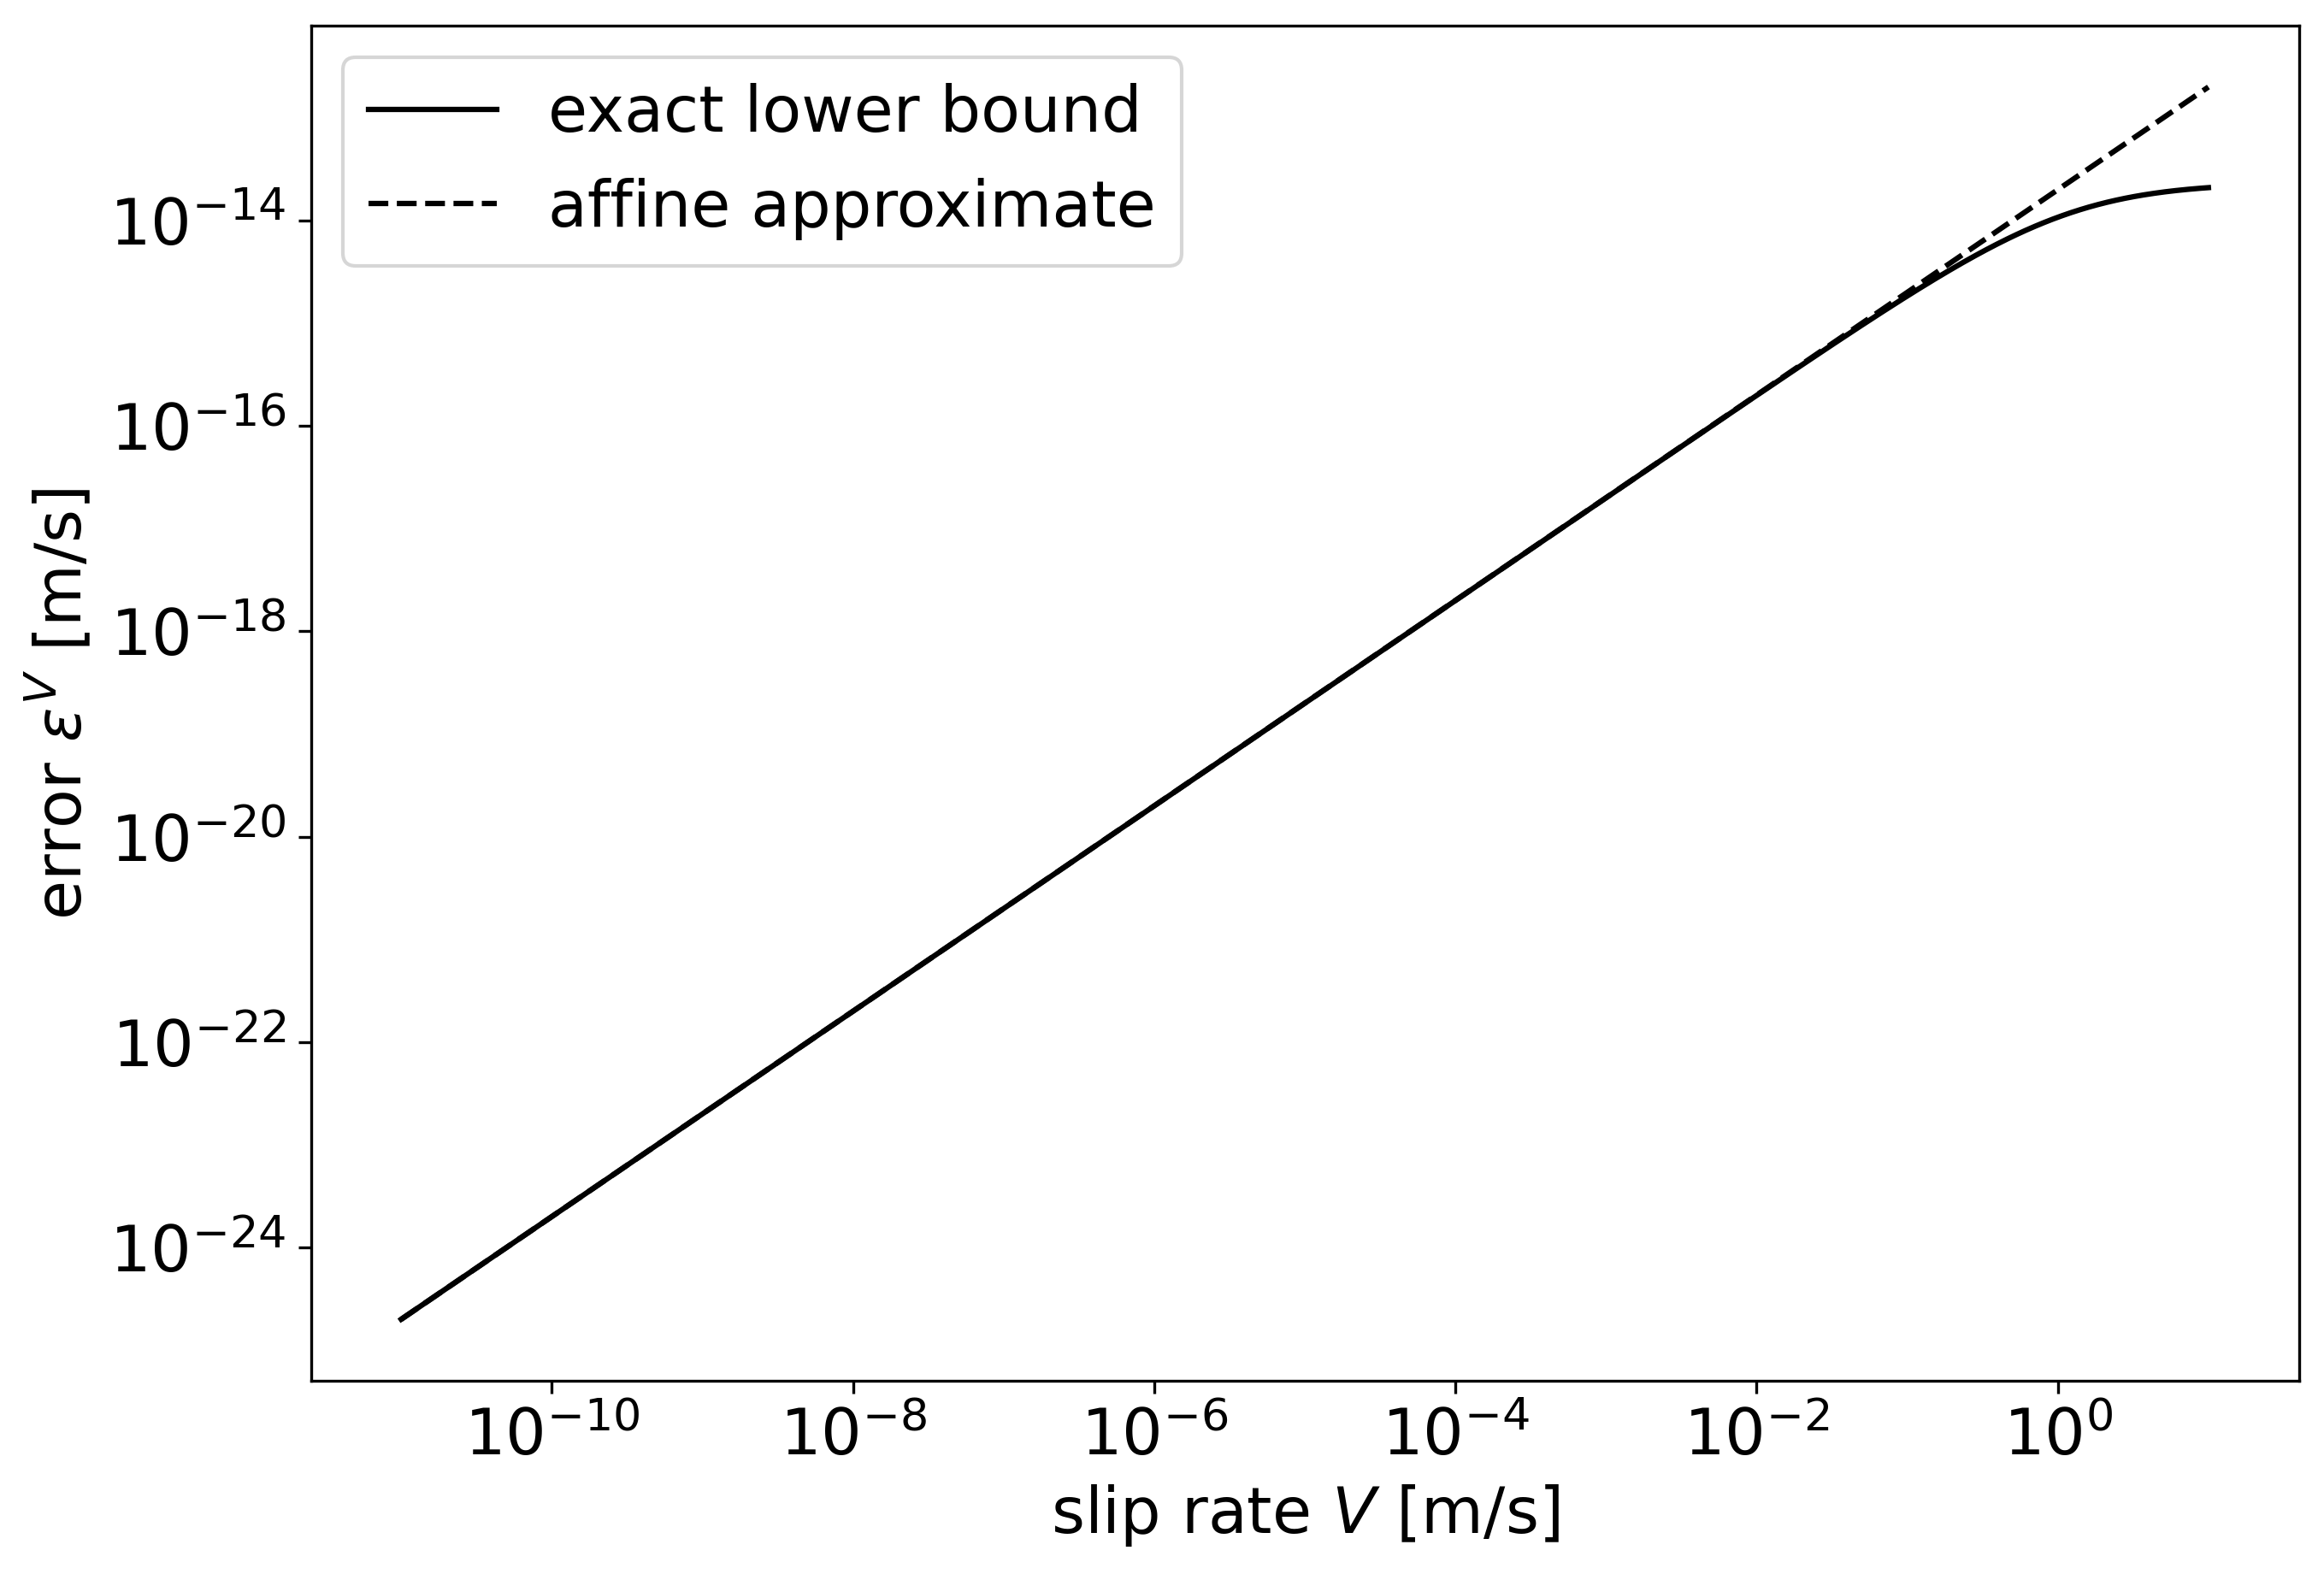
\includegraphics[width=0.5\textwidth]{images/ErrorRelationPSI_VAbsoluteRelative.png}
	\caption{Lower bound for the error in the slip rate $V$ compared to its linear approximate in function of the slip rate}
	\label{fig:LowerBoundErrorEstimateV}
\end{figure}

This section estimated a lower bound for the local truncation error of the different components $\varepsilon^S$, $\varepsilon^\psi$ and $\varepsilon^V$. This means that a tolerance below these values can never be achieved and are an absolute lower bound for $t_i^a$ and $t_i^r$. \\

However, the proposed tolerances are only of theoretical nature, as they assume that the error only stems from the iterative solver of the friction law. However, the time integration would most likely fail because numerical rounding errors or the sum of local truncation errors from the different RK stages have not been considered. Moreover, the error estimate itself is not exact, and, as already discussed in \autoref{ssec:QualityErrorEstimate_0D}, it tends to overestimate the local truncation error, which means that even if the error is within the tolerance, the algorithm would not consider it as such. If one wants to run the simulation with maximal accuracy, it is wise to use larger values than the here presented tolerances.


\section{Newton Iteration}
\label{ssec:ConvergenceNewtonIteration}
The Jacobian matrix is needed to apply implicit numerical methods to the SEAS problem. Unlike explicit methods, they evaluate the right hand side of the ODE with the current solution which is not known yet. To calculate the solution vector at a given timestep, a nonlinear algebraic equation of the form $\varphi(x) = 0$ needs to be solved where $x$ is the solution vector to be determined. The Newton method is often used to solve the equation because of its ease to implement and converges with second order around the solution. 

\begin{itemize}
	\item Calculate an initial guess $x_0$
	\item Repeat until tolerance is reached $\|\phi(x_n)\| < TOL$: 
	\begin{itemize}
		\item $x_{n+1} = x_n - J_\varphi^{-1}(\varphi(x_n)) \varphi(x_n)$
	\end{itemize} 
\end{itemize}

The matrix $J_\varphi^{-1}(f(x_n))$ is the Jacobi matrix of the function $\varphi$ evaluated at the point $x_n$. \\

\subsection{Convergence Properties}
Next, the convergence properties of the Newton iteration with the analytic Jacobian are investigated on the 1st order ODE formulation. For this, we solve one timestep of the implicit Euler method starting from the initial condition of the simulation. The function $\varphi$ and its Jacobian matrix are given by:
\begin{align}
\varphi(x) &= -x + x^{(0)} + h \Gamma(x) \\
J(x) &= -I + h J_\Gamma(x)
\end{align}
The vector $x$ contains both the components related to the slip $S$ and to the state variable $\psi$ and the right-hand side vector $\Gamma(x)$ contains their respective time derivative. The Jacobian of the proposed Newton iteration needs the Jacobian $J_\Gamma(x)$ of the right-hand side vector, of which the correctness is evaluated here. The success of the Newton iteration, thus to measure second-order convergence, also indicates the correctness of the Jacobian matrix. \\
Furthermore, the behavior of the analytic expression of the Jacobian is compared to the behavior of an iterative approximation of it. Broyden's method \cite{BroydenIteration} provides an enhancement of the Newton method which updates the Jacobian matrix at each iteration without the need of its analytical expression. The main difficulty lies in finding an appropriate initial guess to achieve fast convergence. 

\begin{itemize}
	\item Calculate the initial guesses $x_0$ and $J_0$
	\item Repeat until tolerance is reached $\|\varphi(x_n)\| < TOL$: 
	\begin{itemize}
		\item $\Delta x_n = x_n - x_{n-1}$ and $\Delta \varphi_n = \varphi(x_n) - \varphi(x_{n-1})$ 
		\item $J_n = J_{n-1} + \frac{\Delta \varphi_n - J_{n-1}\Delta x_n}{\|\Delta x_n\|^2} \Delta x_n^T$
		\item $x_{n+1} = x_n - J_n \varphi(x_n)$
	\end{itemize} 
\end{itemize}

The motivation behind this update scheme is to minimize the Frobenius norm $\|J_n~-~J_{n-1}\|_F$. As a matter of simplicity, the initial guess of the Jacobian is obtained with the analytical expression of it, even though its correctness has not yet been shown. Other initialization methods such as finite differences do not lead to convergence of the Broyden method. \\
The experiment has been performed on a symmetric, two-dimensional domain of varying size. The initial guesses for $x$ are obtained with one step of the explicit Euler method with a timestep of $h = 10^5$s. This timestep is large enough to obtain an error to the exact value at this time which requires several Newton iterations to be corrected but remains small enough to ensure that the Newton iteration converges at all. The evolution of the residual $\varphi(x_n)$ is shown in \autoref{fig:convergenceNewtonAndBroydenDifferentSizes}.

\begin{figure}[H]
	\centering
	\begin{subfigure}{0.45\textwidth}
		\centering
		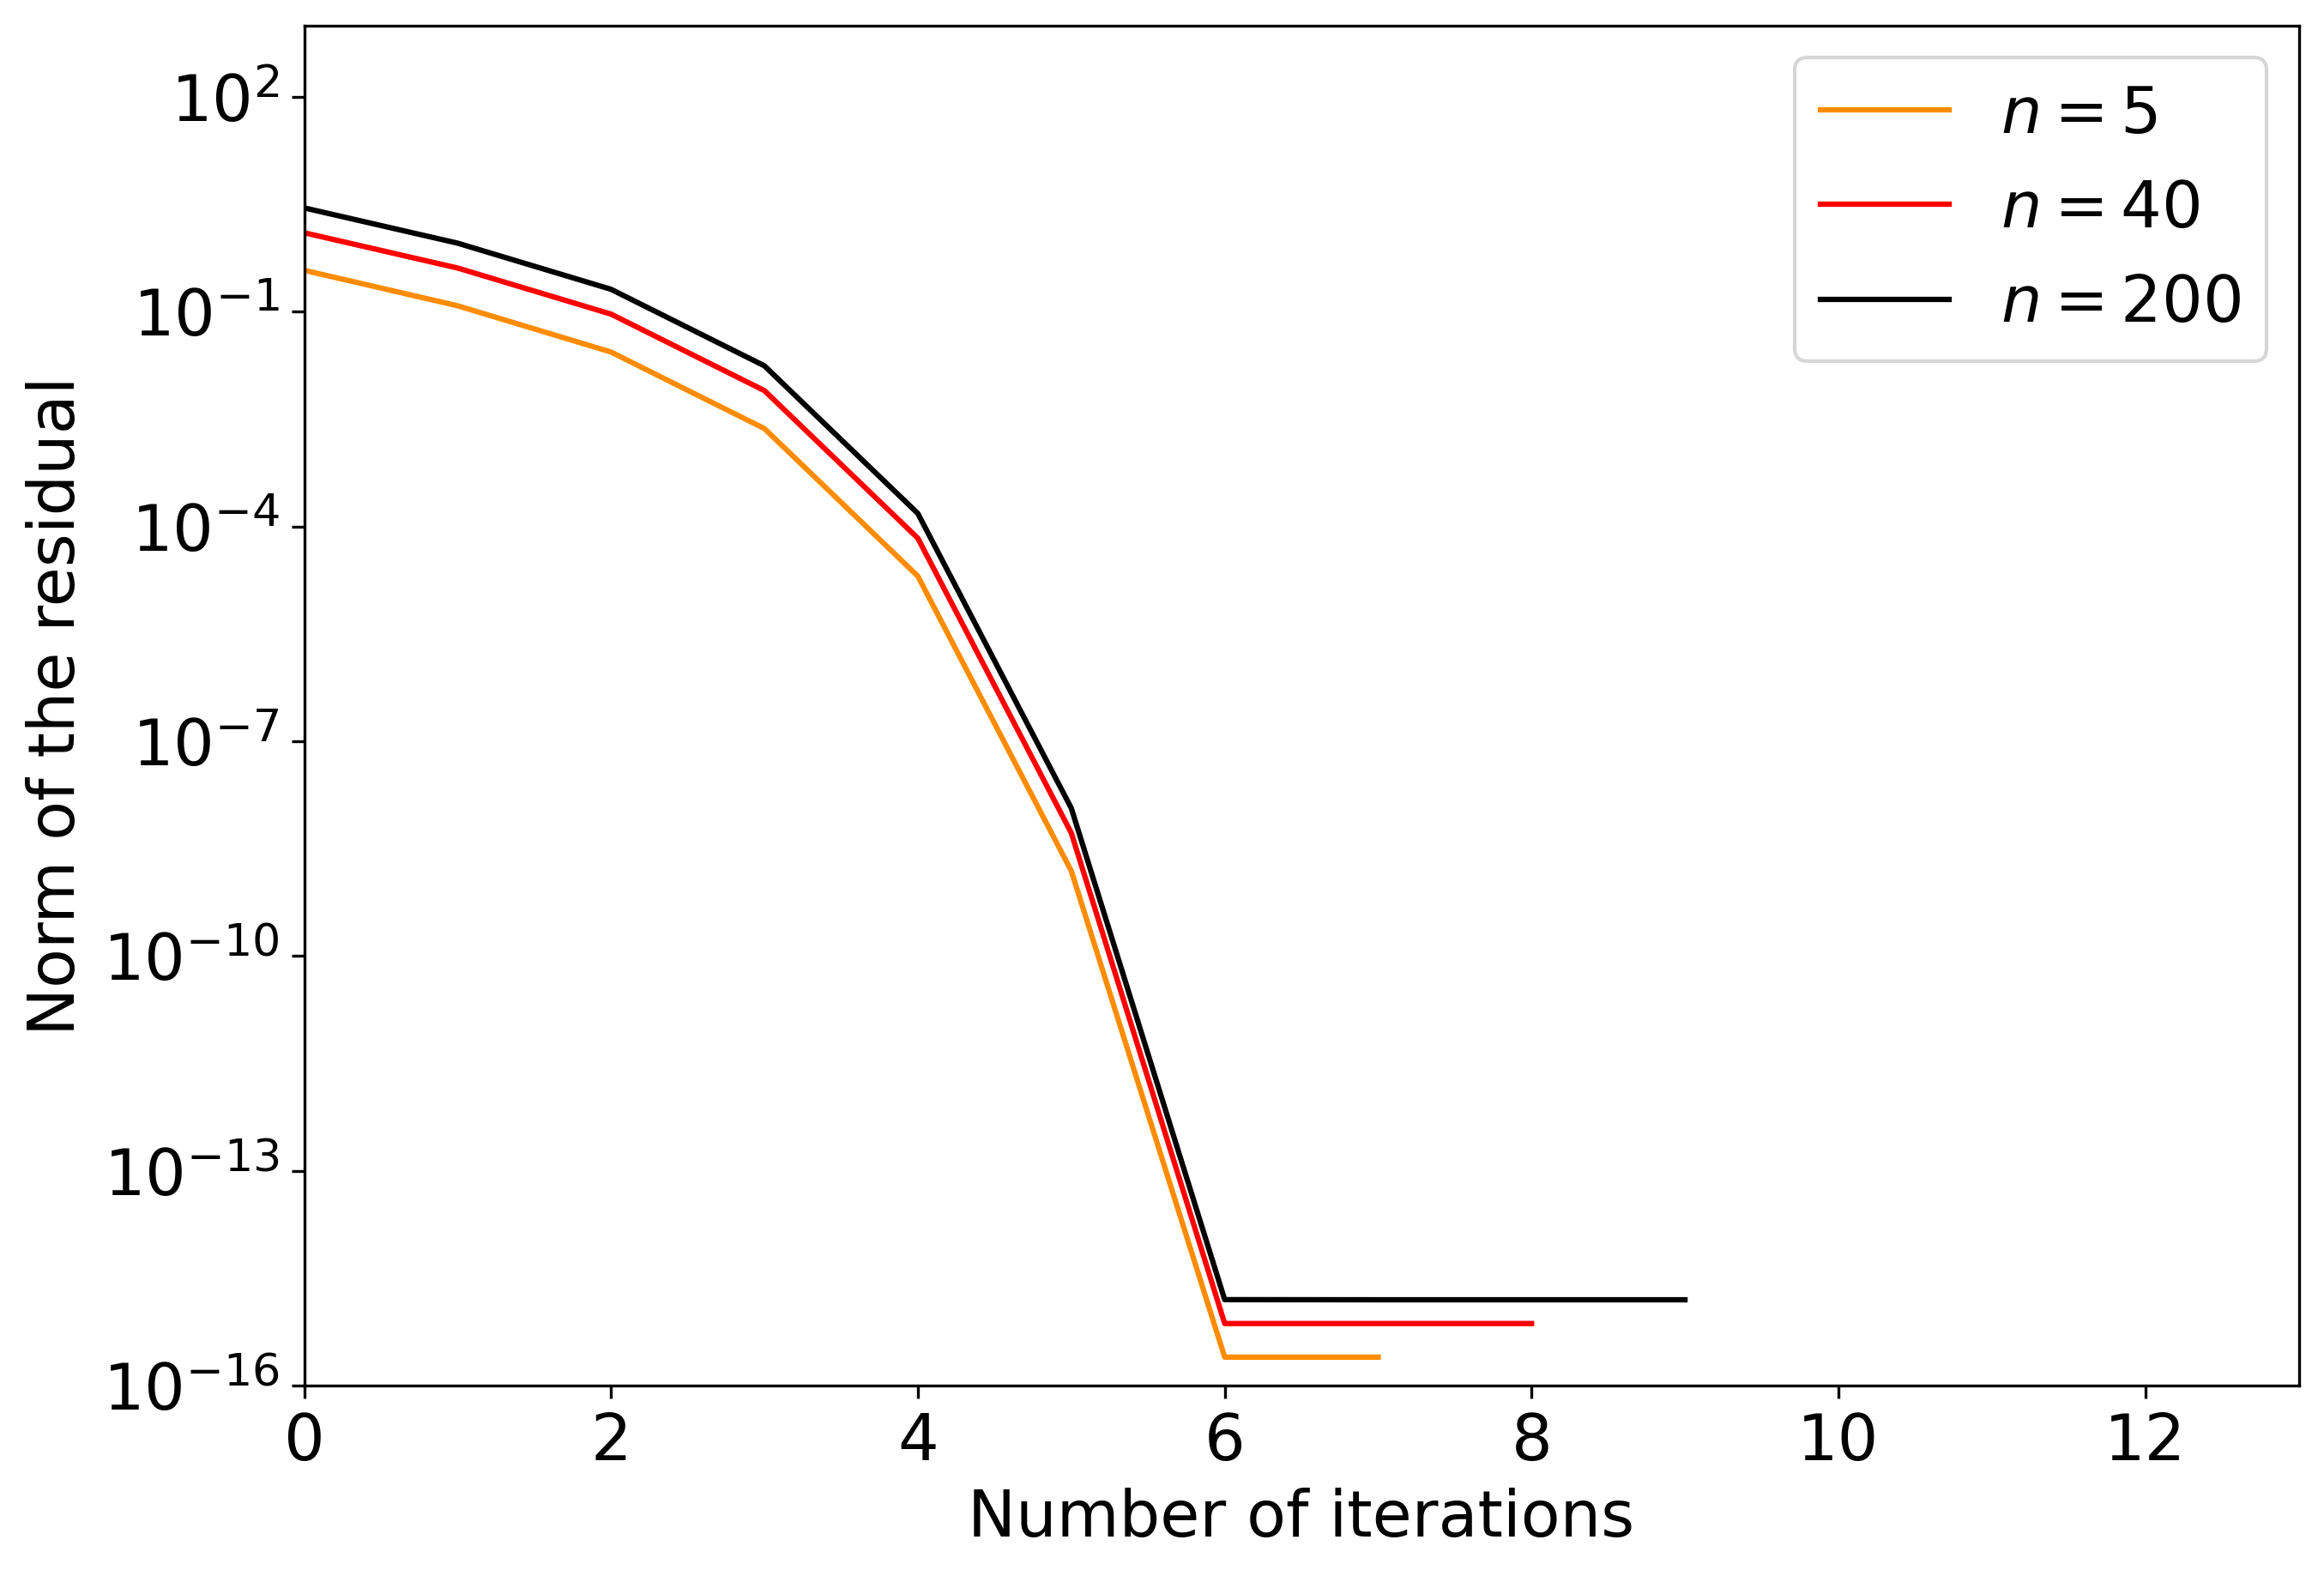
\includegraphics[width=1\textwidth]{images/NewtonIterationConvergenceDT1e5_DifferentSizes_Analytic.png}
		\subcaption{Direct iteration}
	\end{subfigure}
	\begin{subfigure}{0.45\textwidth}
		\centering
		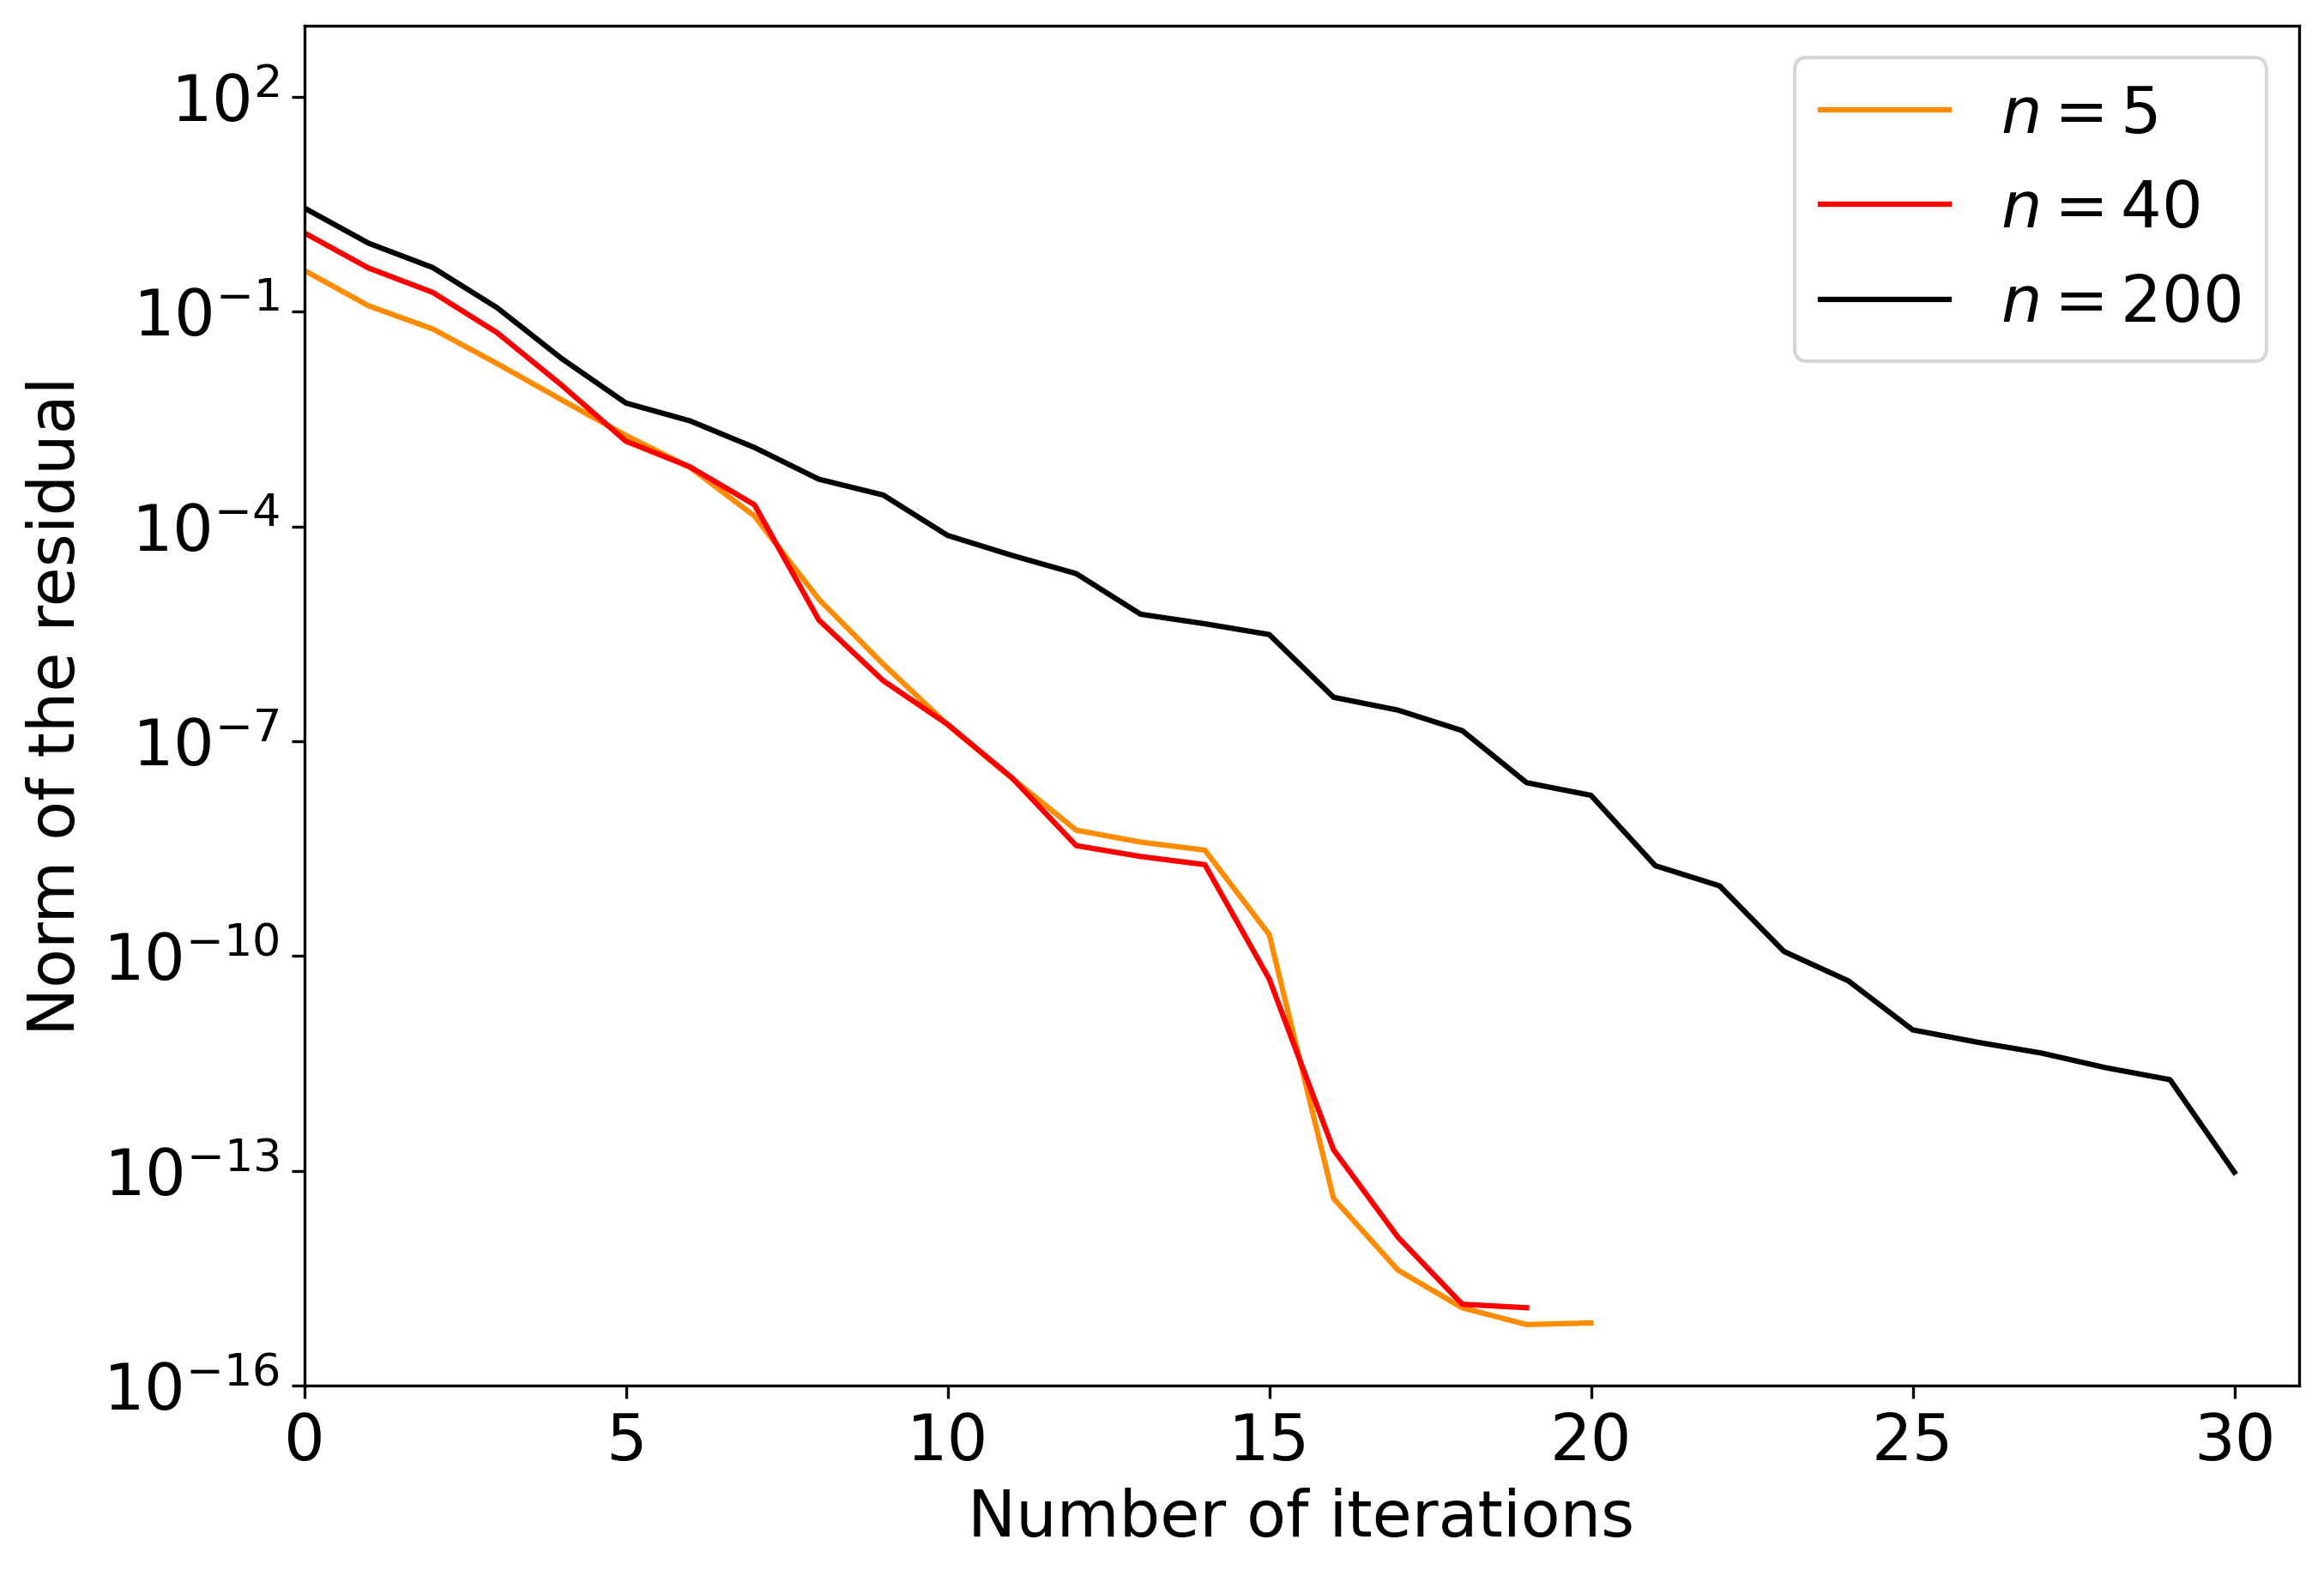
\includegraphics[width=1\textwidth]{images/NewtonIterationConvergenceDT1e5_DifferentSizes_Broyden.png}
		\subcaption{Broyden iteration}
	\end{subfigure}
	\caption{Evaluation of the L2 norm of the residual $\varphi(x_n)$ at each iteration of the Newton and Broyden methods for a timestep size of $h=10^5$s and for different problem sizes $n$}
	\label{fig:convergenceNewtonAndBroydenDifferentSizes}
\end{figure}

It can be immediately seen that the Newton method with an analytic expression of the Jacobian reaches the maximum reachable accuracy of about $10^{-15}$ much faster than if it was approximated with the Broyden method. The convergence rate even seems to be quadratic, as one would expect for the Newton iteration and the convergence is similarly fast for all tested domain sizes. The Broyden method on the other hand shows rather a linear convergence behavior, and the number of needed iterations increases with problem size. This makes the Broyden iteration particularly unsuitable for simulations on large domains. The approximated Jacobian matrix at the end of the Broyden iteration matches with high precision its analytic counterpart since the maximum relative difference among the entries is of the order of $10^{-5}$. \\
So far, it has been shown that the Newton iteration converges well for various domain sizes. The chosen timestep size $10^5$s is still small, as, in the aseismic slip, it may reach the order $10^7$s. \autoref{fig:convergenceNewtonAndBroydenDifferentTimeSteps} shows the norm of the residual for the timestep sizes $10^5$s, $10^6$s and $10^7$s. The direct iteration with the analytic Jacobian matrix always has a quadratic convergence, and the slightly higher number of iterations for large timesteps is essentially caused by the worse initial guess. In contrast, the Broyden iteration converges much slower if the timestep size increases. 
\begin{figure}[H]
	\centering
	\begin{subfigure}{0.45\textwidth}
		\centering
		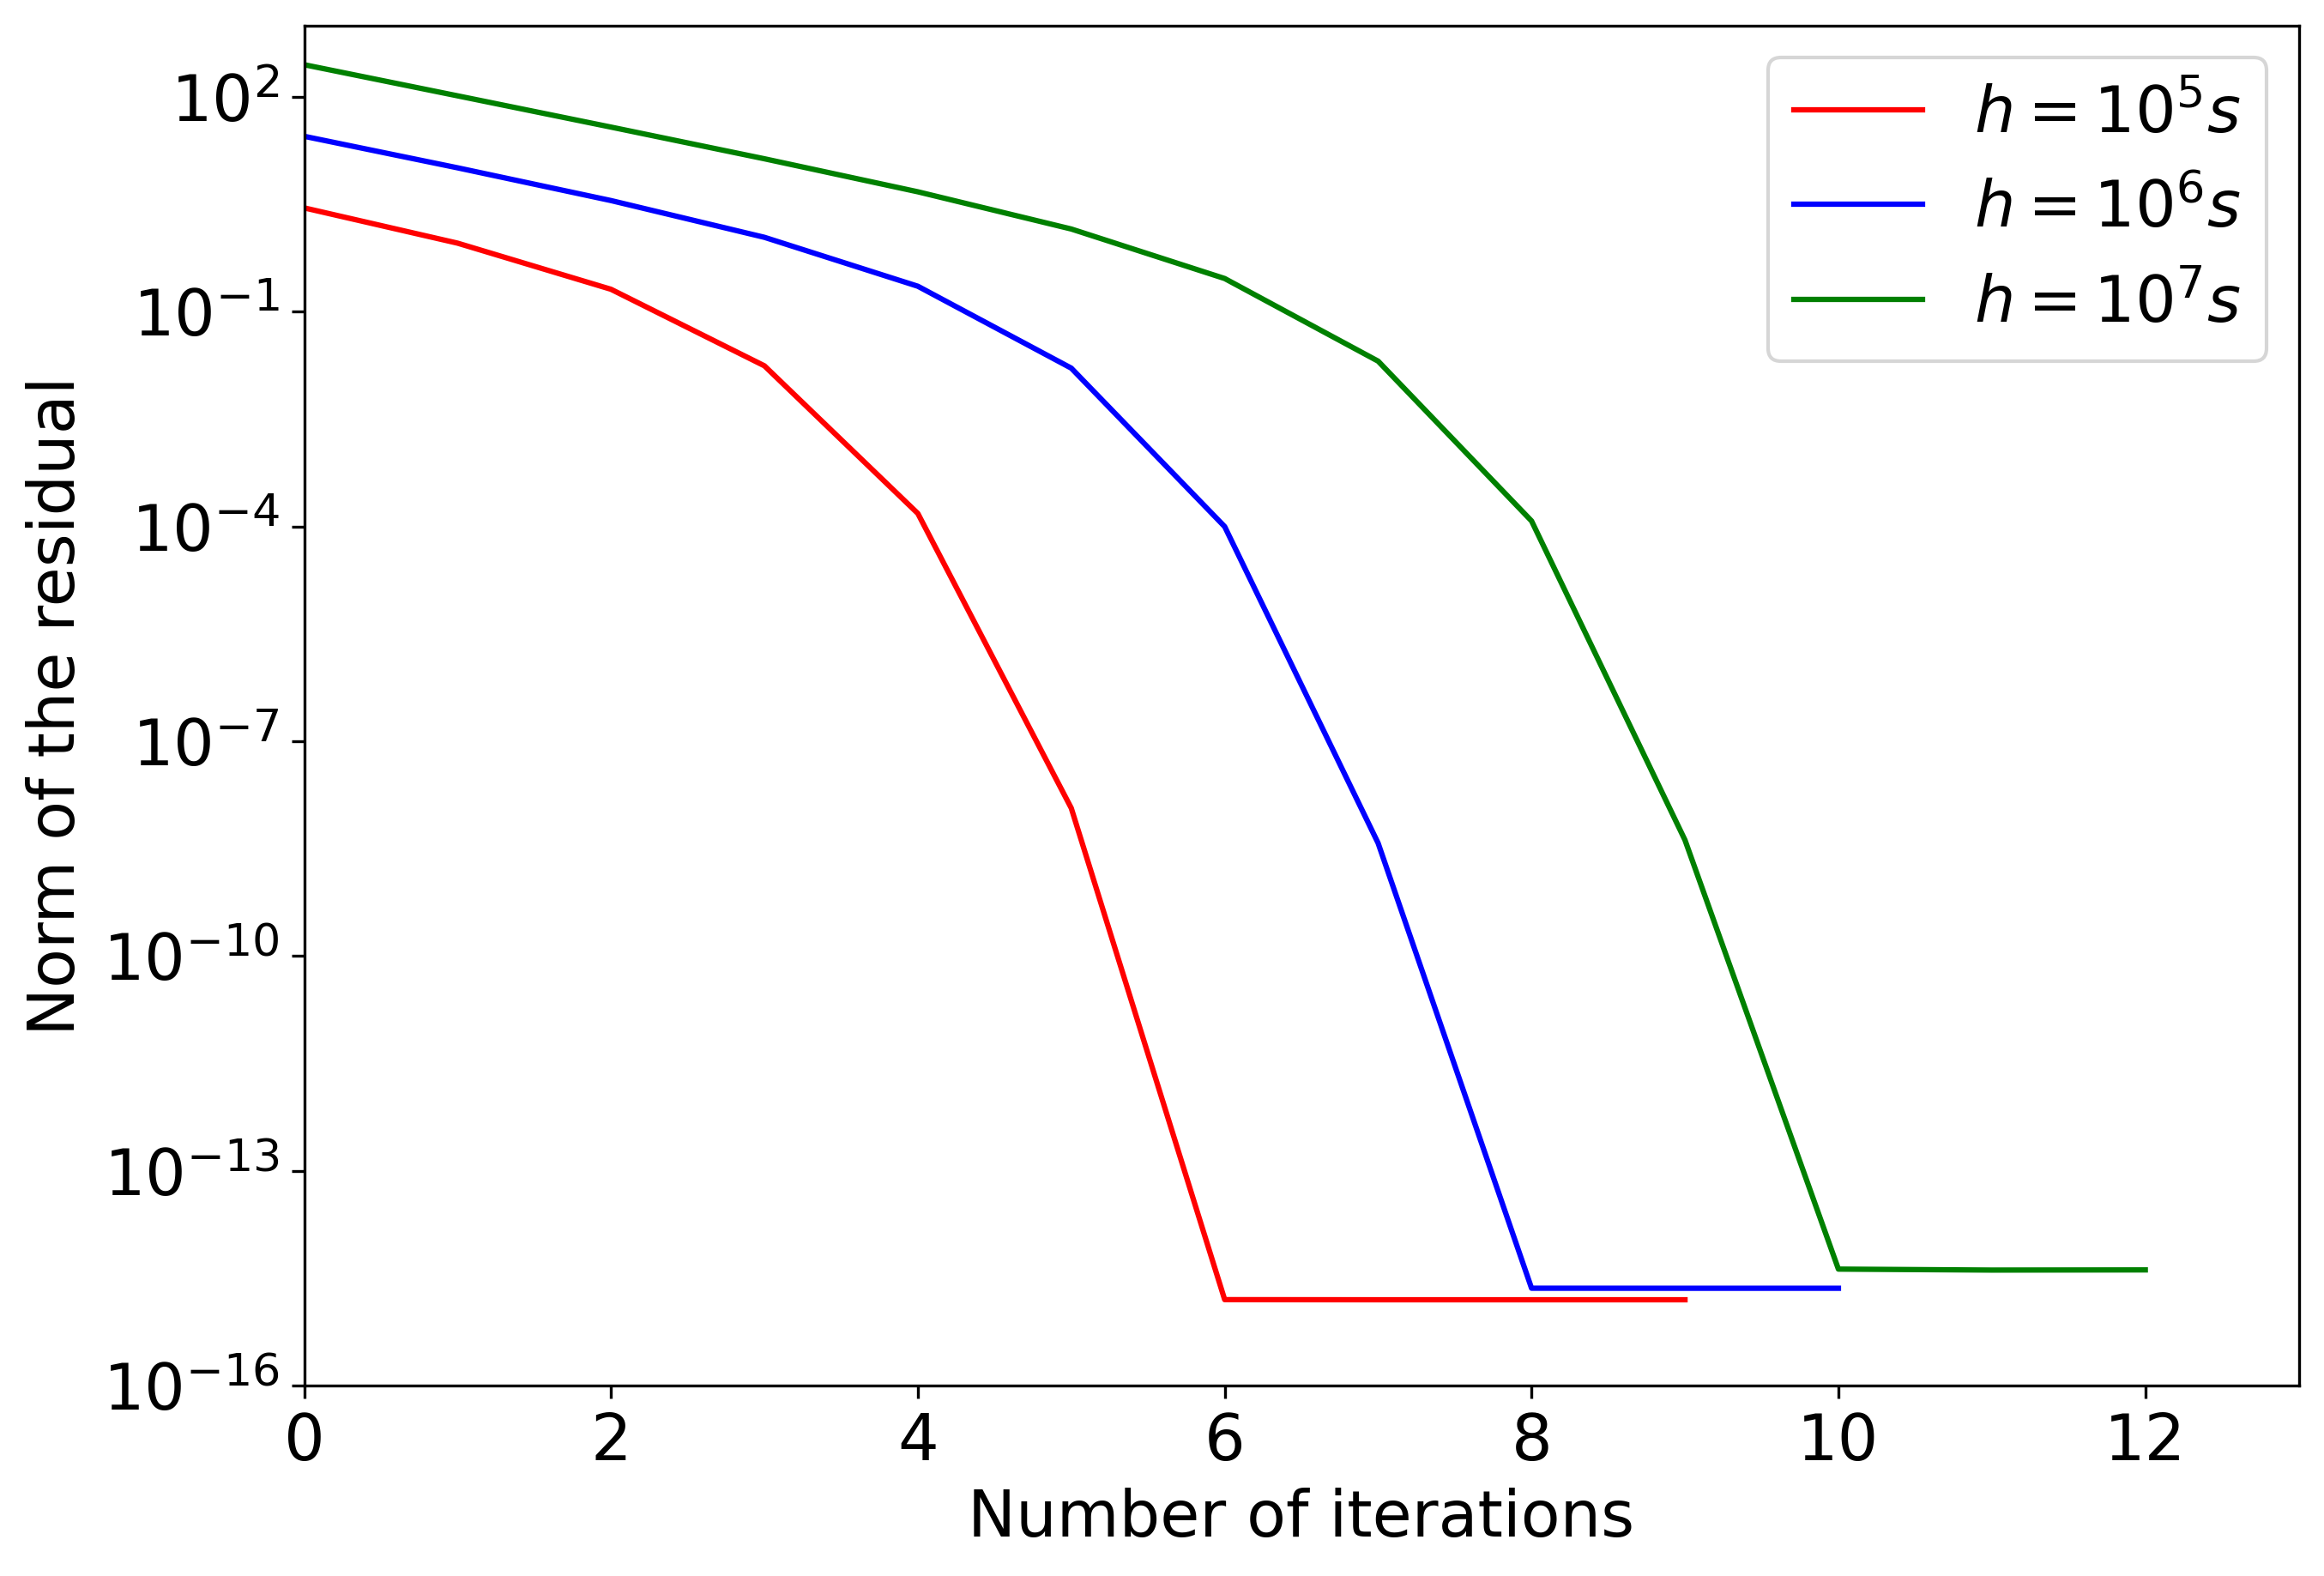
\includegraphics[width=1\textwidth]{images/NewtonIterationConvergence200Elements_DifferentDT_Analytic.png}
		\subcaption{Direct iteration}
	\end{subfigure}
	\begin{subfigure}{0.45\textwidth}
		\centering
		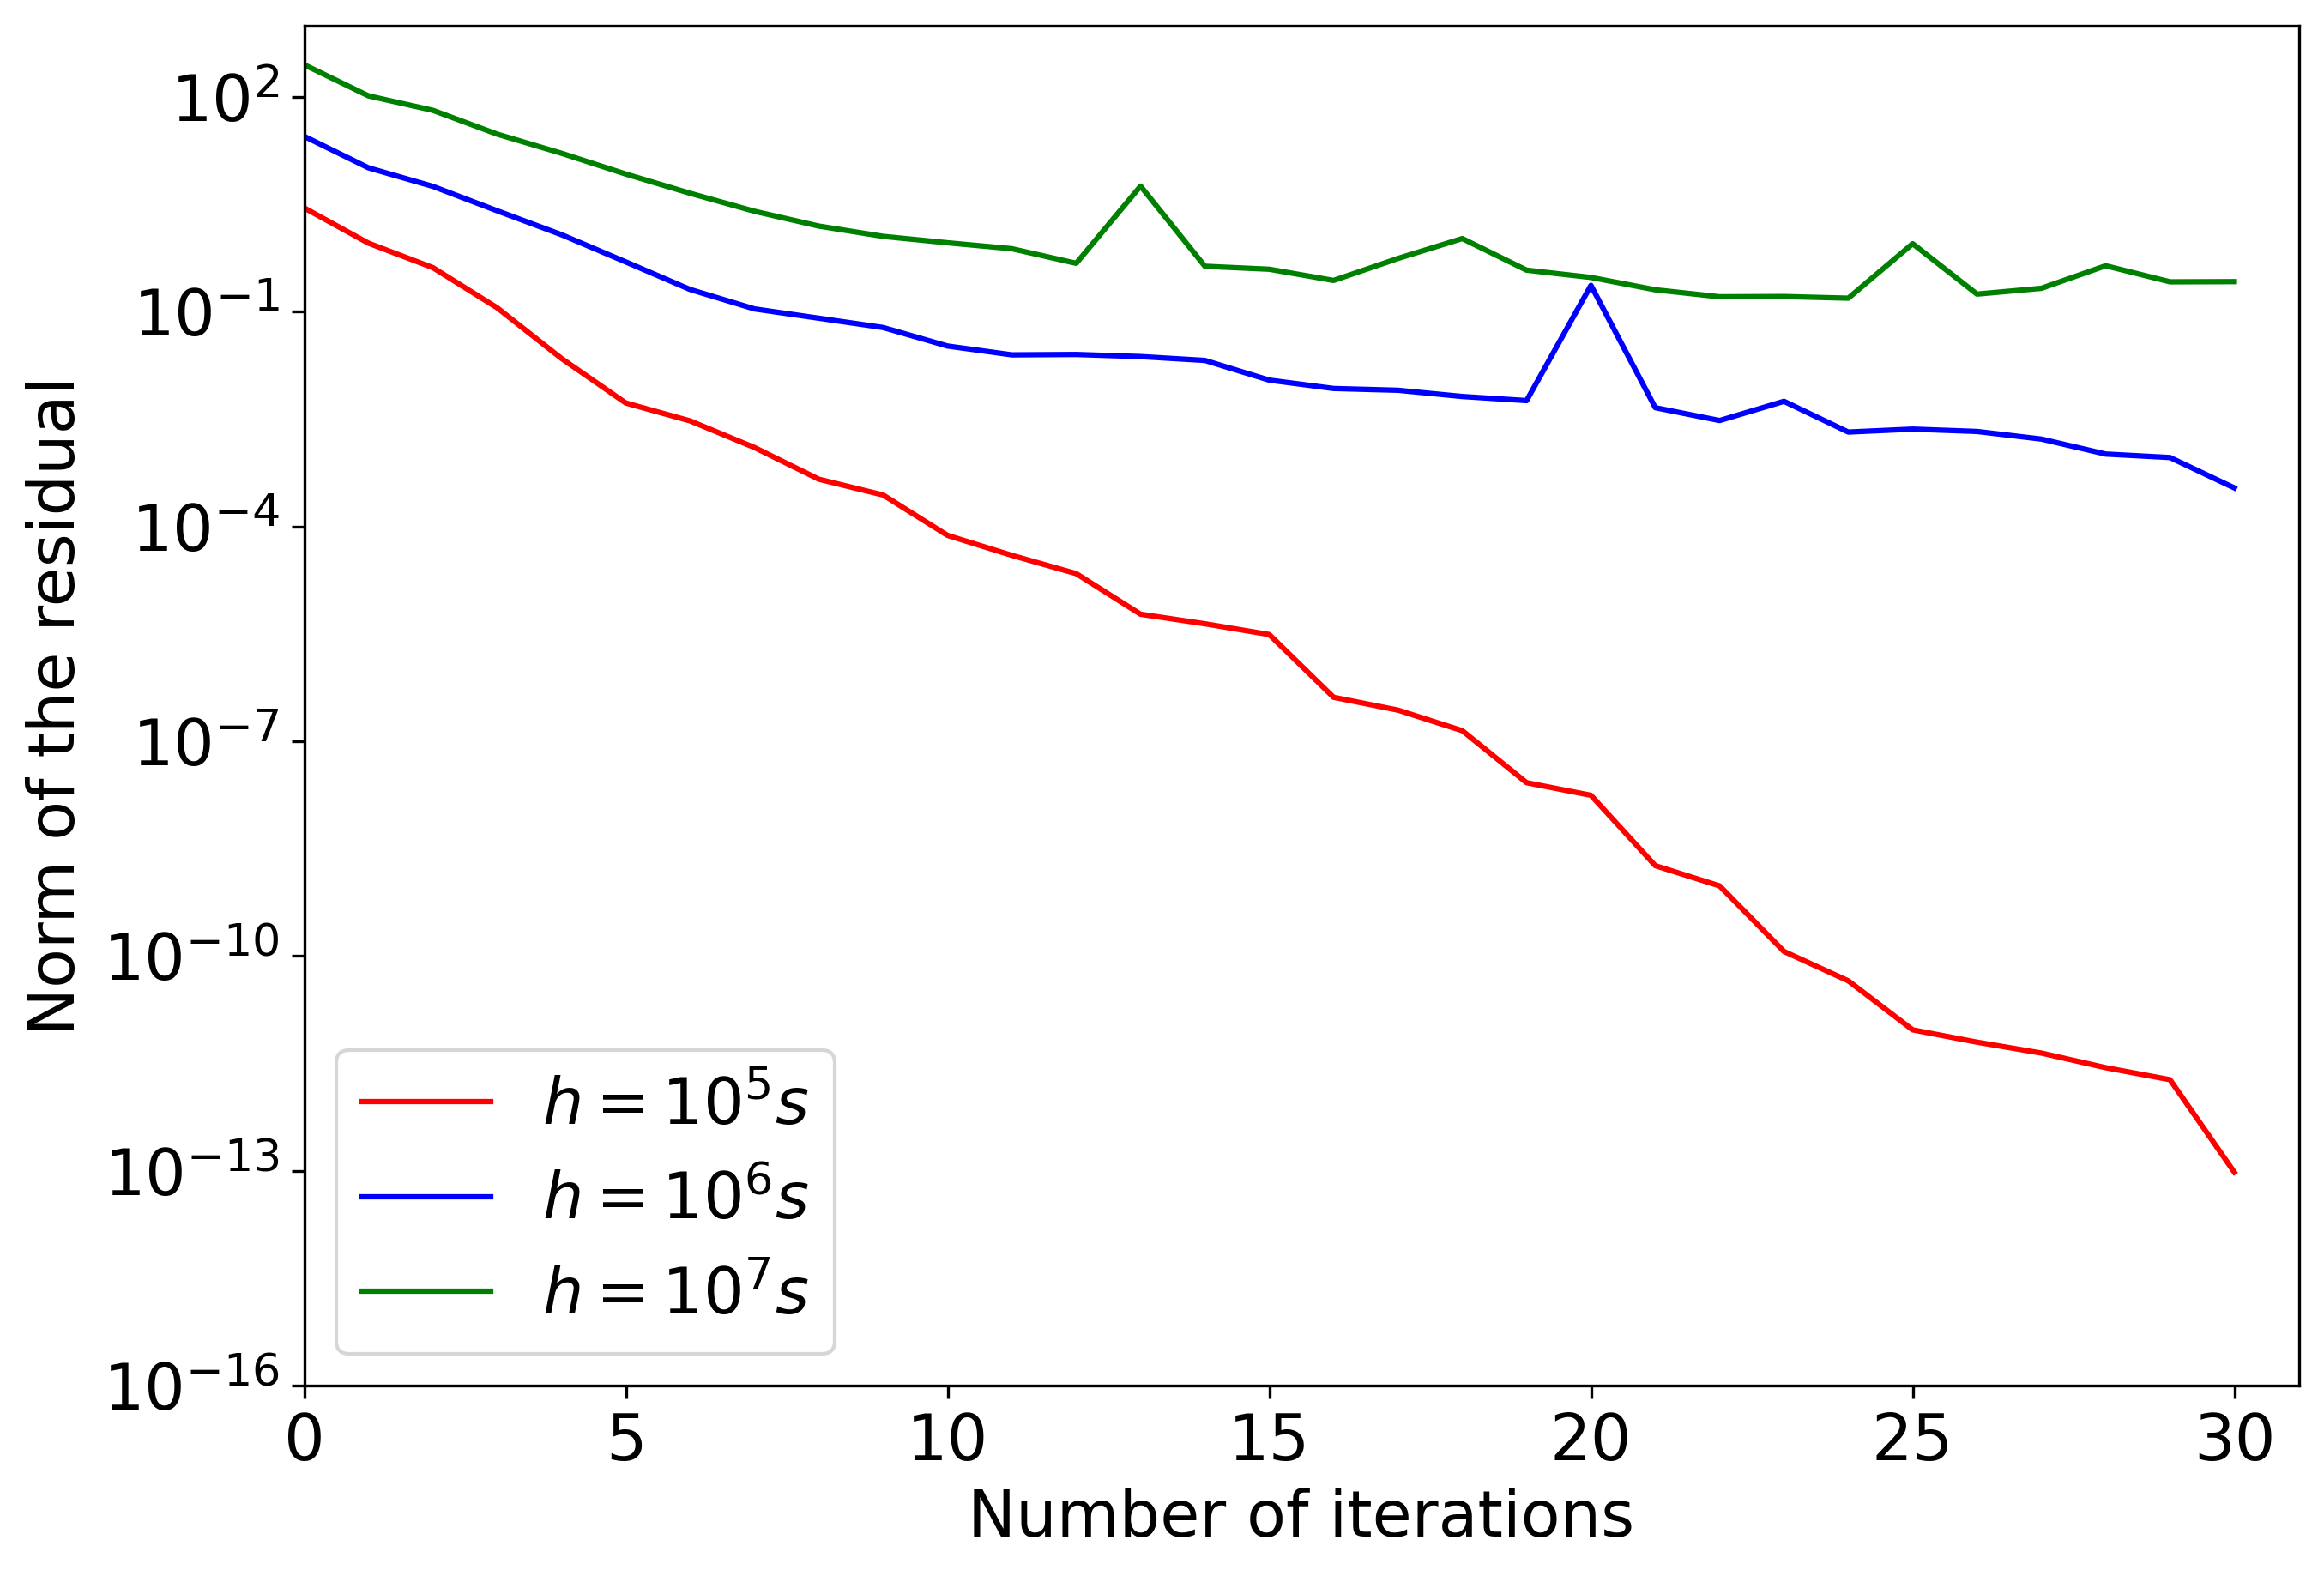
\includegraphics[width=1\textwidth]{images/NewtonIterationConvergence200Elements_DifferentDT_Broyden.png}
		\subcaption{Broyden iteration}
	\end{subfigure}
	\caption{Evaluation of the L2 norm of the residual $\varphi(x_n)$ at each iteration of the Newton and Broyden methods on a domain with 200 fault elements for different timestep sizes $h$}
	\label{fig:convergenceNewtonAndBroydenDifferentTimeSteps}
\end{figure}

It was shown that the Newton iteration with the analytic Jacobian has excellent convergence properties for any domain sizes and large timestep sizes. On the other hand, the alternative with a Broyden iteration, which approximates the Jacobian matrix along with the solution, converges only very slowly for large domains and large timesteps which is why this method is not suited to solve the problem. In practice, the  Newton iteration converges much faster because BDF schemes of higher order are used instead of the implicit Euler and the initial guess at the beginning of the iteration is obtained by extrapolating the previous solution vectors to the current simulation time. Usually, one Newton step is required to achieve the desired accuracy, which means two evaluations of the right-hand side function. \\

\subsection{Convergence issues with the compact DAE formulation}
The compact DAE formulation from \autoref{eq:DAE_compact_formulation_SEAS} shows a similar convergence behavior only during the aseismic slip. Whereas the method never diverges, the maximal achievable accuracy depends on the current timestep size, in a way that for very small timesteps, the residual in the Newton iterations does not go below some large value. Convergence to a non-optimal stationary point can be seen in \autoref{fig:convergenceIssuesCompactDAENewtonIterations}, which shows the infinity norm of the residual at each Newton step for different timestep sizes. The largest instance, of the order $10^7$, is representative of the aseismic slip after the first earthquake and the other samples have been taken in the initial phase of the second earthquake when the slip rate increases significantly and the timestep size decreases. \autoref{fig:convergenceIssuesCompactDAEMaxResidual_vs_dt} shows the maximum residual at the end of the Newton iteration in function of the current timestep size for all timesteps in the simulation. The locations of the samples in the first graph are highlighted by colored points. It can be seen that a large residual norm inversely depends on the timestep size. \\ 

\begin{figure}[H]
	\centering
	\begin{subfigure}[t]{0.32\textwidth}
		\centering
		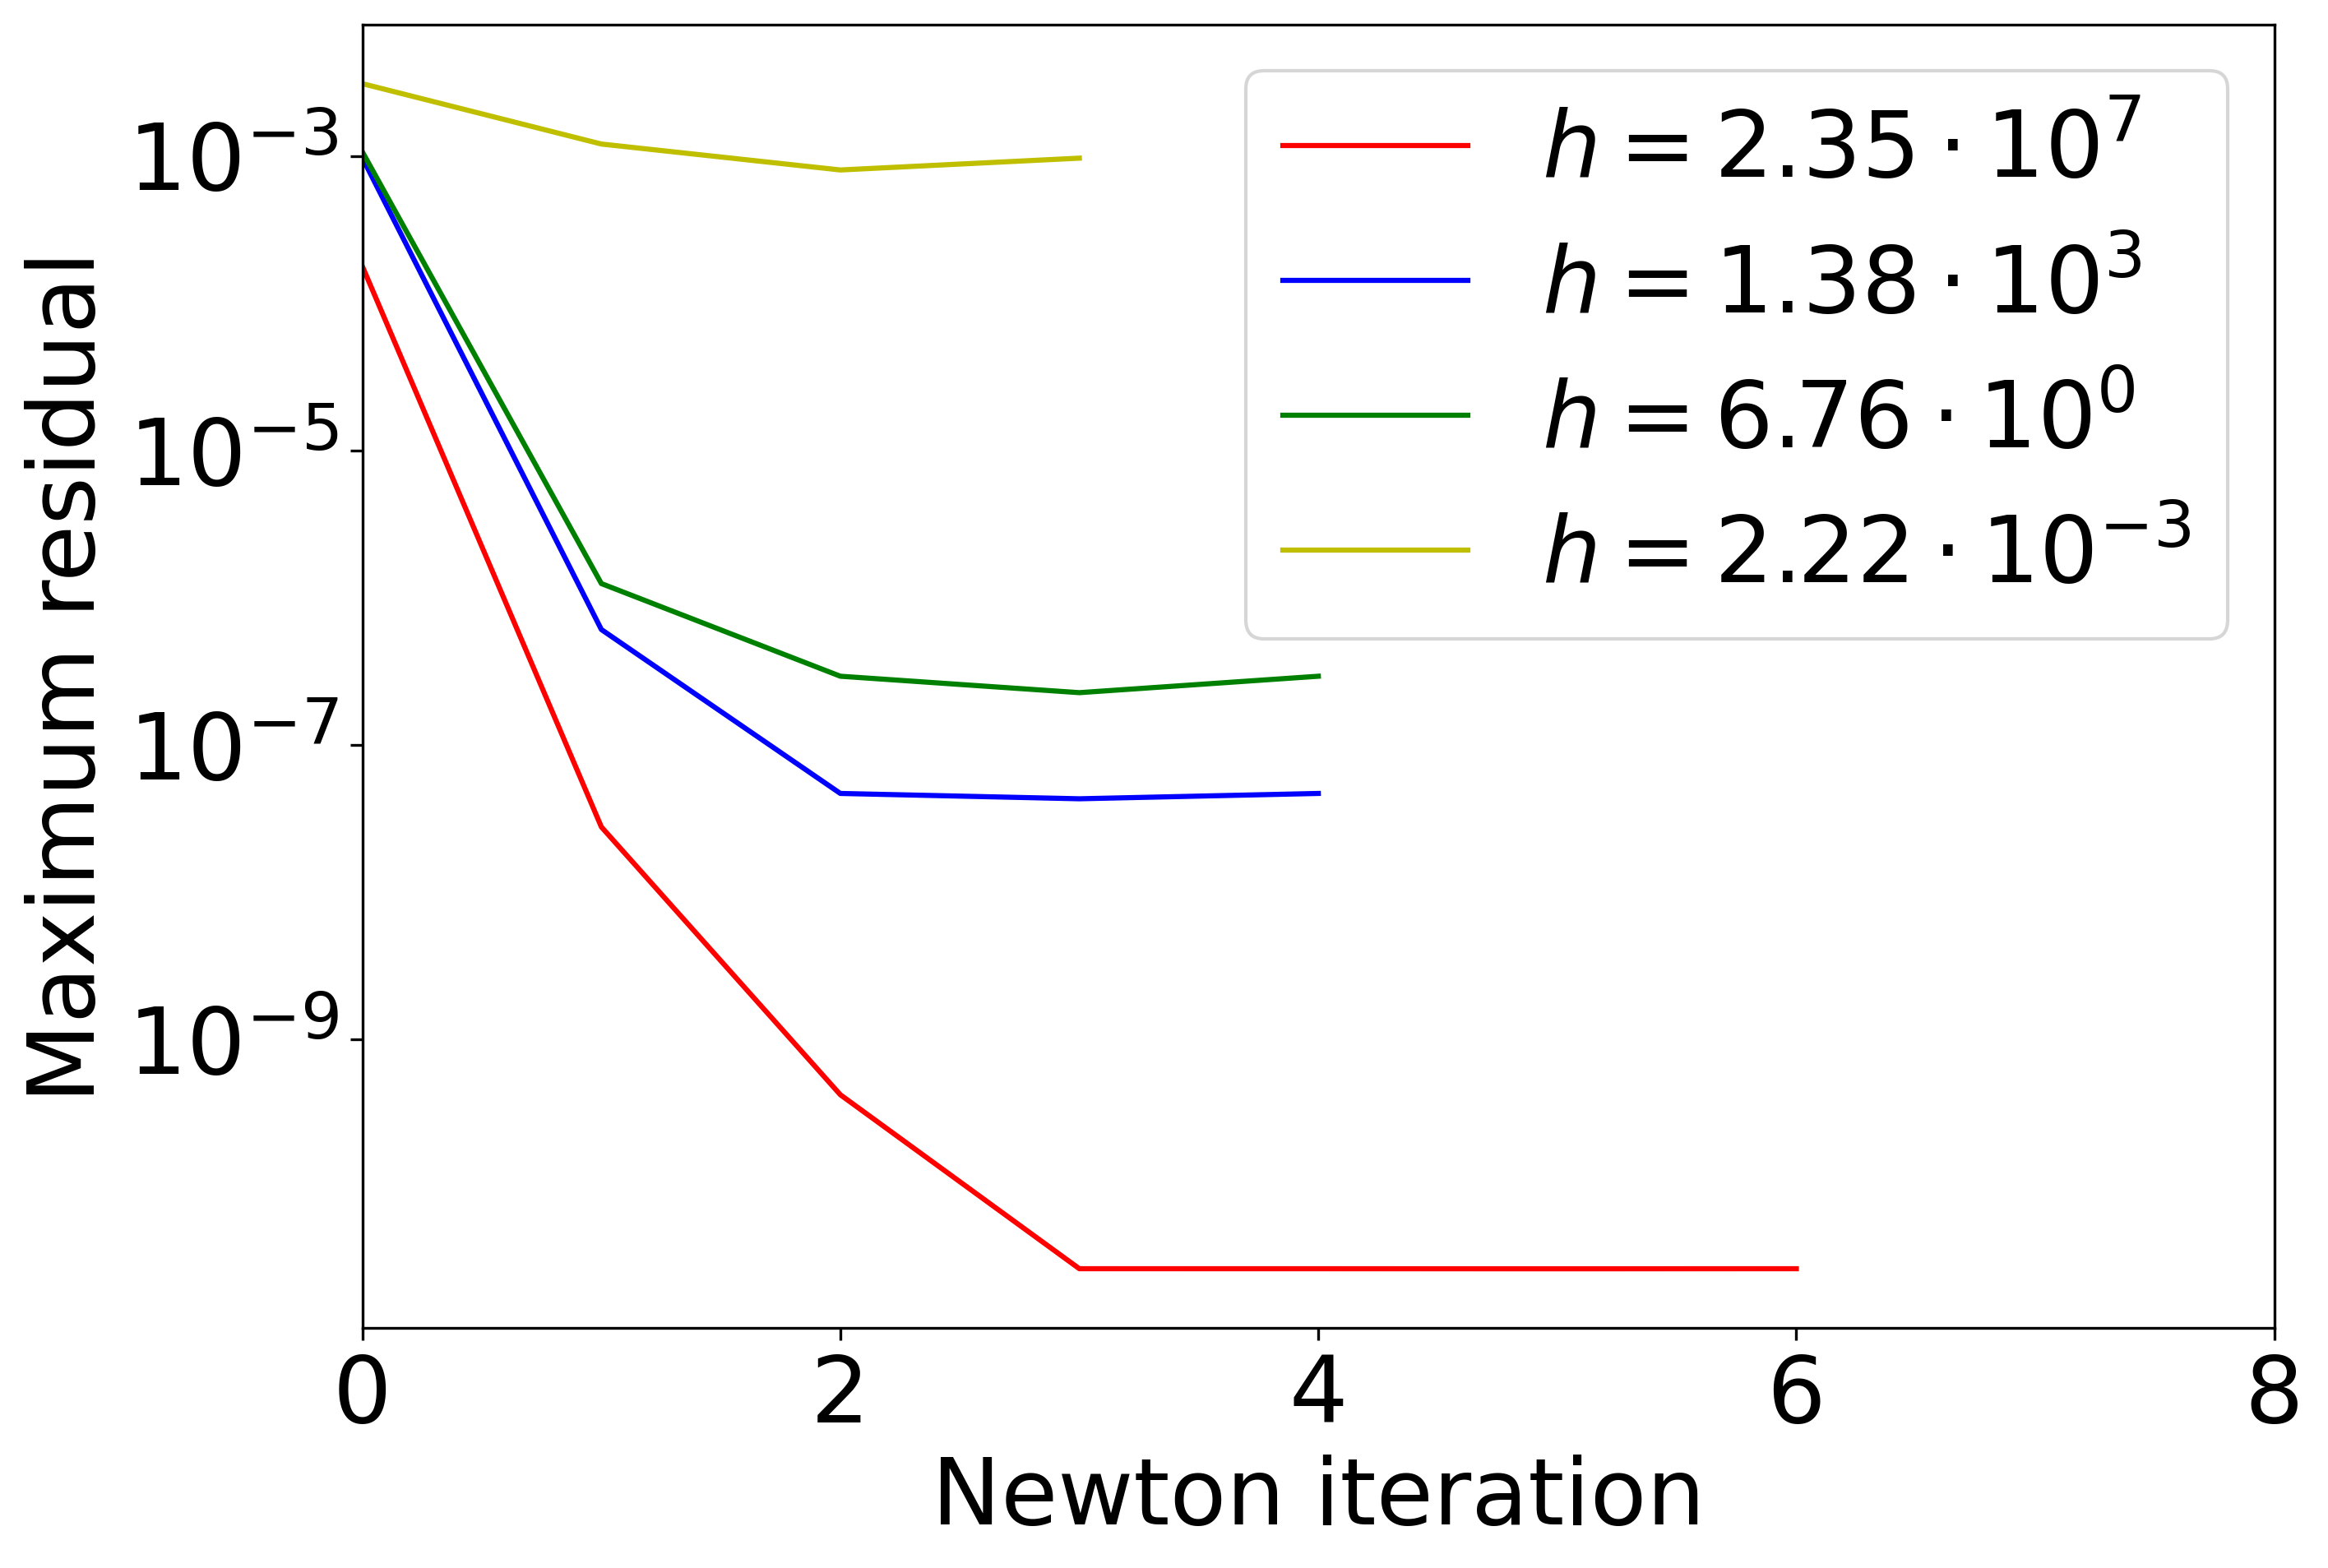
\includegraphics[width=0.9\textwidth]{images/TANDEMConvergenceAnalysisCompactDAENewton_Size5.png}
		\subcaption{$\infty$-norm of the residual in the Newton iterations at different timestep sizes}
		\label{fig:convergenceIssuesCompactDAENewtonIterations}
\end{subfigure}
	\begin{subfigure}[t]{0.32\textwidth}
		\centering
		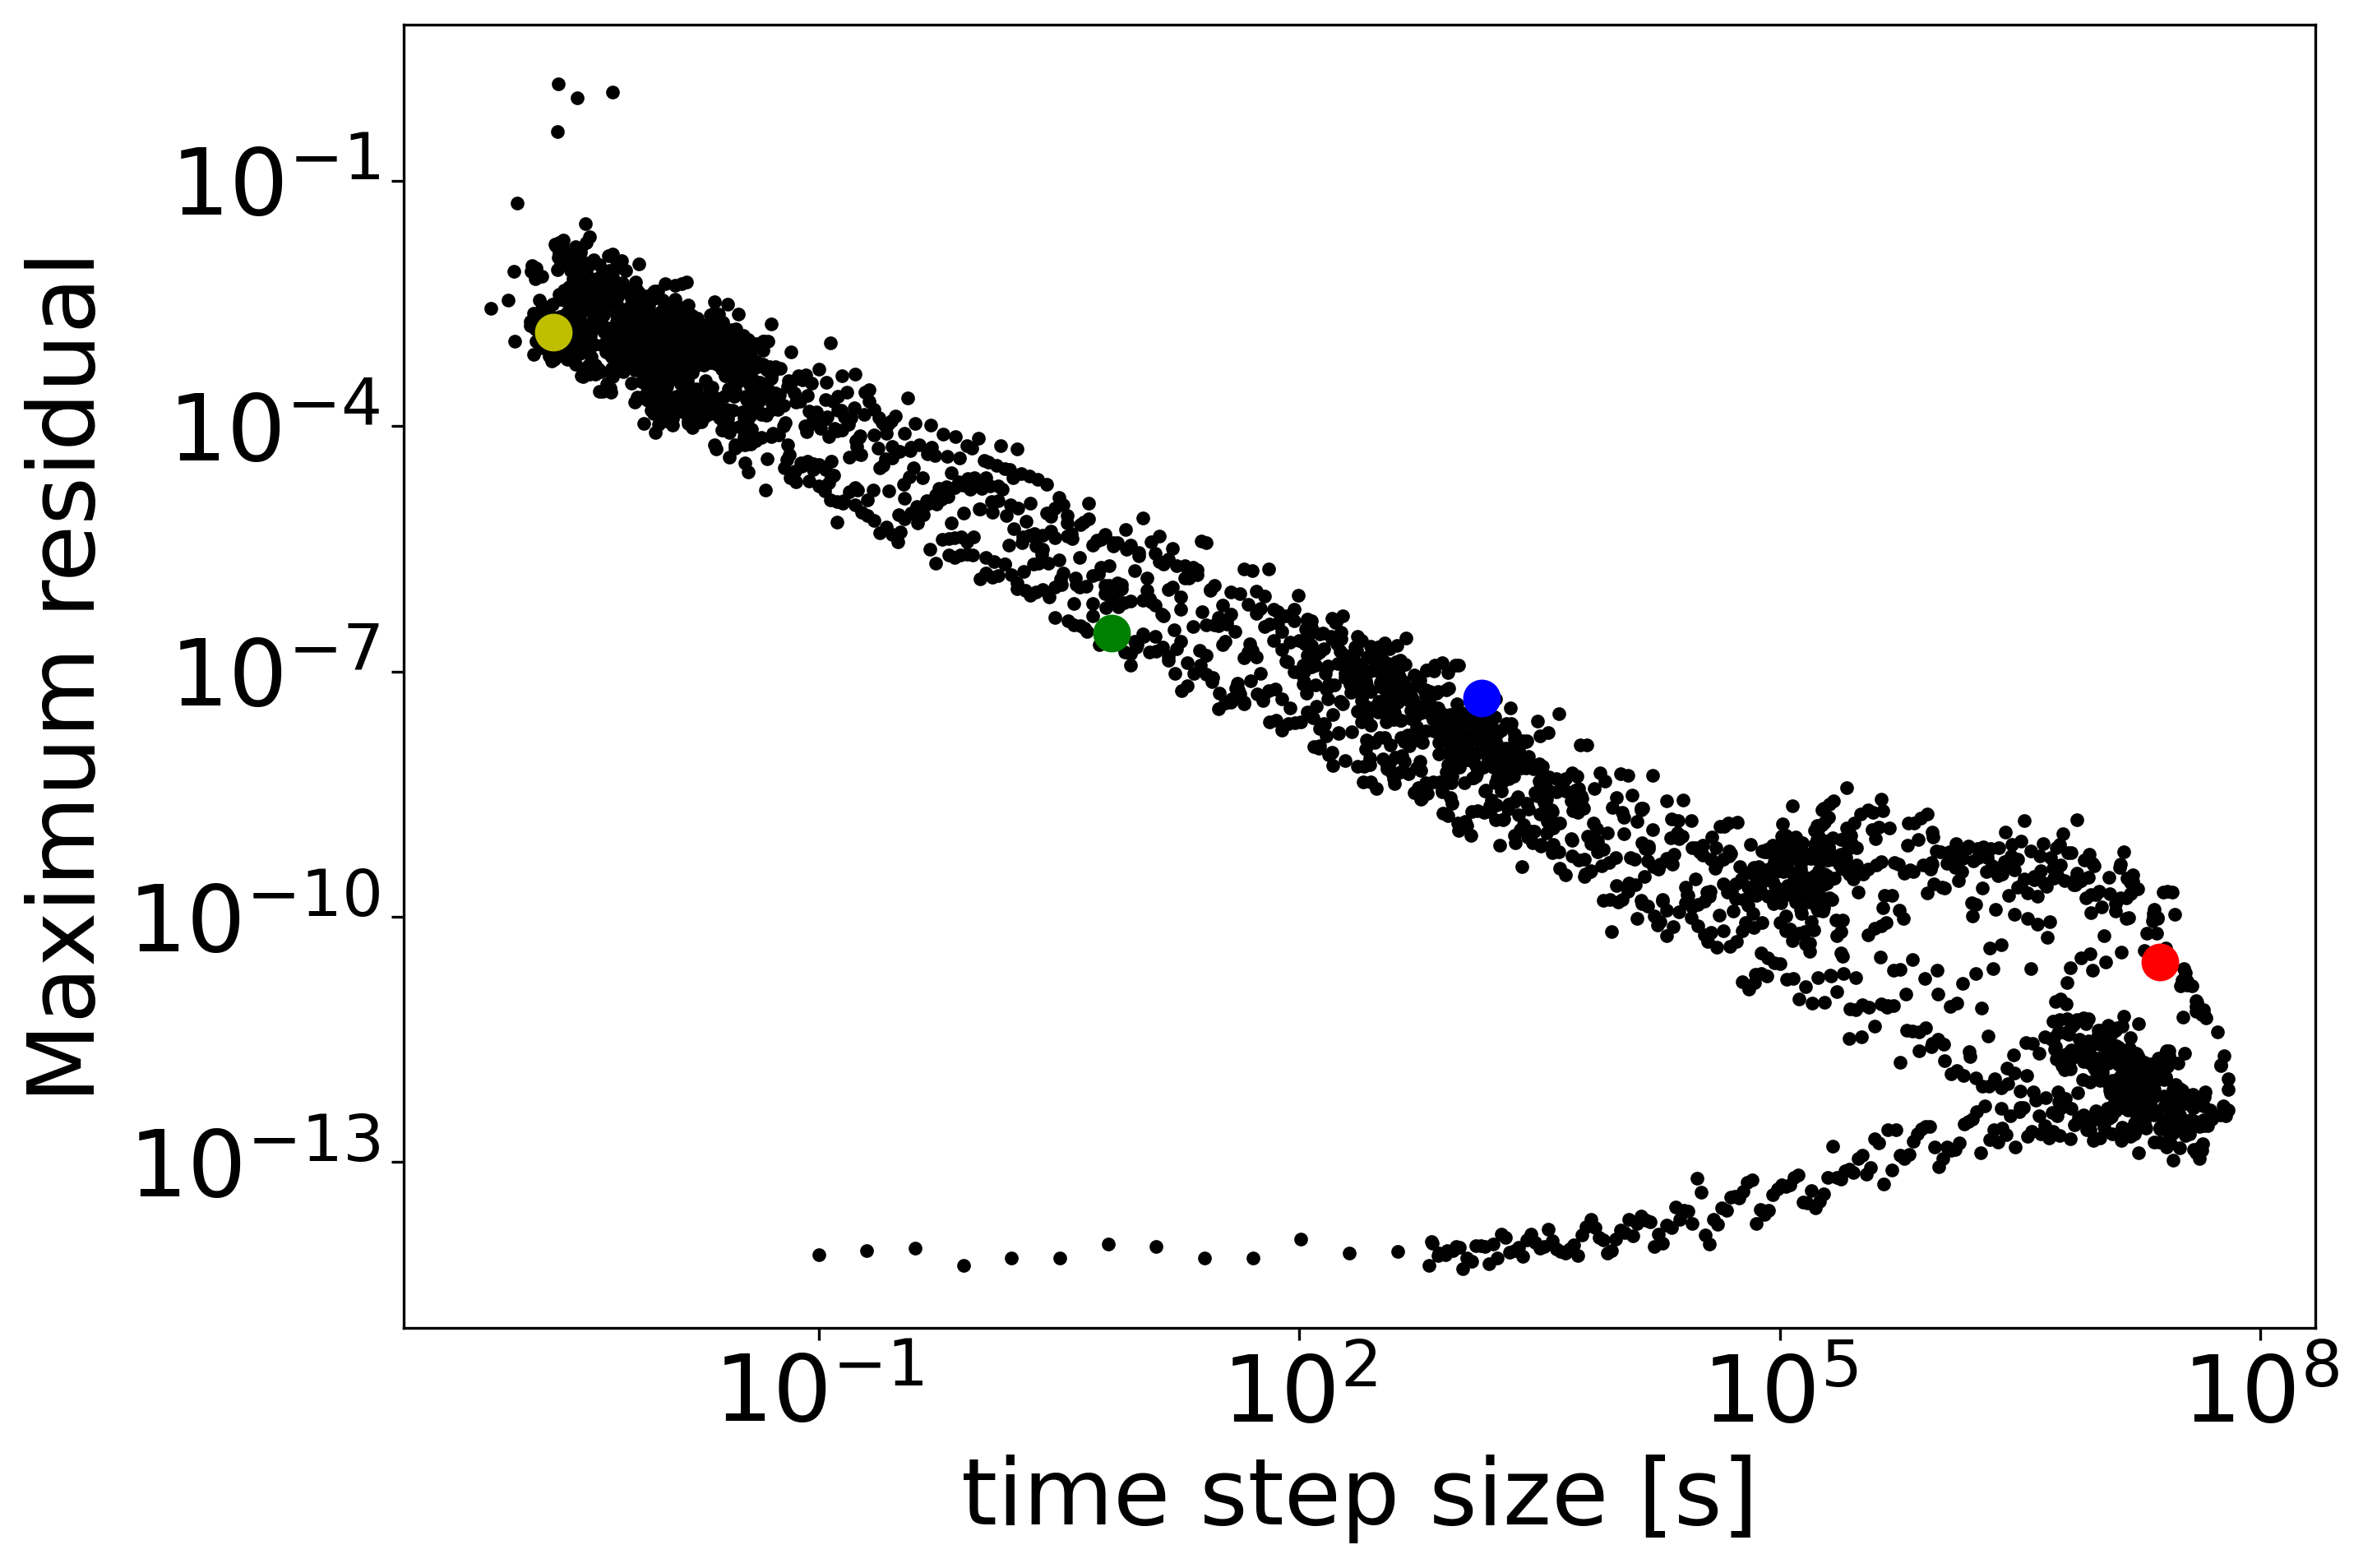
\includegraphics[width=1\textwidth]{images/TANDEMConvergenceAnalysisCompactDAEMaxResidual_Size5.png}
		\subcaption{Minimum achievable residual norms in function of the timestep size}
		\label{fig:convergenceIssuesCompactDAEMaxResidual_vs_dt}
	\end{subfigure}
	\begin{subfigure}[t]{0.32\textwidth}
		\centering
		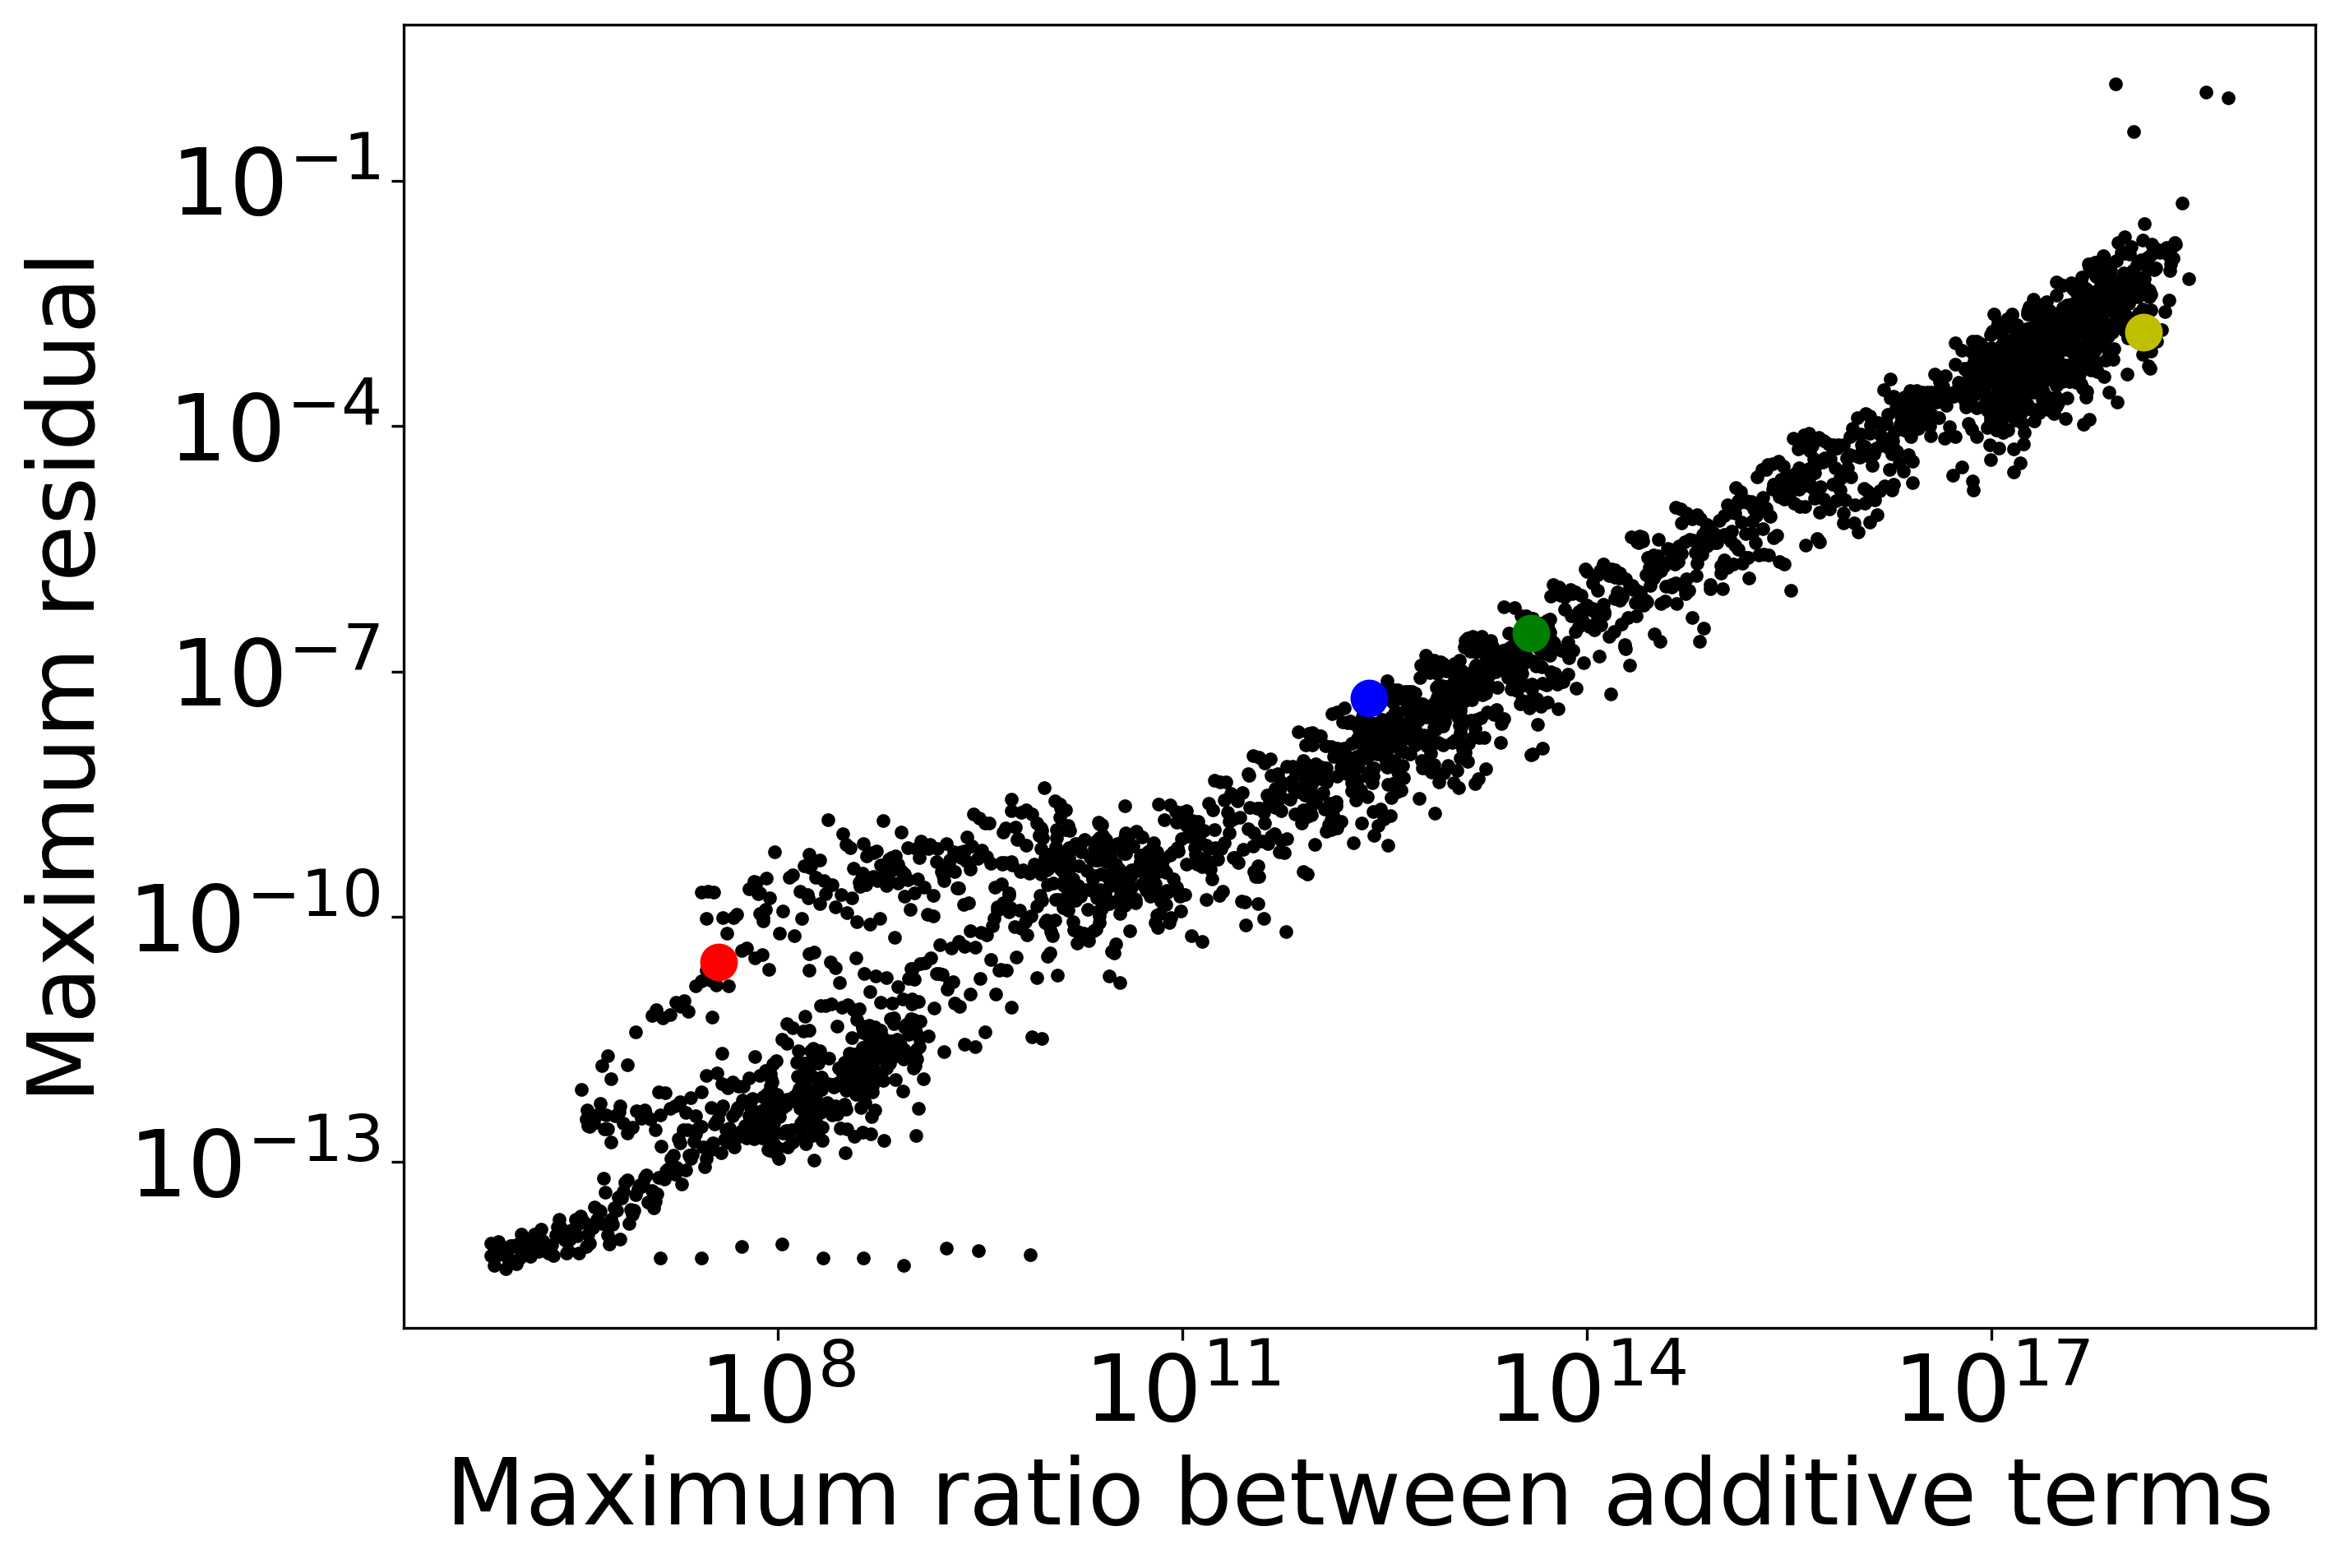
\includegraphics[width=1\textwidth]{images/TANDEMConvergenceAnalysisCompactDAERatioInAddition_Size5.png}
		\subcaption{Minimum achievable residual norms in function of the maximal ratio between the additive terms in the Jacobian matrix}
		\label{fig:convergenceIssuesCompactDAEMaxResidual_vs_ratio}
	\end{subfigure}
	\caption{Convergence properties of the compact DAE formulation with the 4th order BDF method on a small domain with 5 fault elements}
\end{figure}
To obtain these results, the time integration itself has not been performed with the compact DAE formulation since it yields a poor accuracy, but rather with the 1st order ODE formulation using a classic adaptive RK4 scheme. At each timestep, the Newton iteration has been performed until the residual norm does not decrease anymore and the final result was discarded. Therefore, the solution vectors at the previous timesteps needed in the BDF method stem from the explicit RK4 time integration and thus slightly differ to the vectors in the time integration with the compact DAE formulation. In a discussion of the convergence this difference is not significant, since the convergence issues arise in either case. \\

The reason for this poor convergence can be found in the definition of the Jacobian matrix of the compact DAE formulation in \autoref{eq:Jacobian_compact_DAE}. As a quick reminder, the Jacobian matrix in the Newton iteration is obtained by $\mathbf{J} = \bm{\Phi}_x + \sigma \bm{\Phi}_{\dot{x}}$, where the shift $\sigma$ depends on the order $k$ of the BDF scheme and on the timestep sizes in  $k$ previous timesteps. The upper left block in the Jacobian is thus the sum of $\sigma\pdv{F}{V}$ and $\pdv{F}{S}$. The first partial derivative is of the magnitude $10^9$ in the aseismic slip and reaches values up to the order $10^{15}$ in an earthquake. On the other hand, the second summand takes values between $10^0$ and $10^2$. Since the former is a diagonal matrix, the sum only affects the diagonal elements. Since the timestep size does not change significantly after one timestep, it can be assumed that it is of the same order of magnitude as in the previous timestep. The shift $\sigma$ is then of the order $\sigma = \Theta\left(h_n^{-1}\right)$, where $h_n$ is current timestep size. In the aseismic slip, $\sigma$ is thus of the order $10^{-7}$ and can go as high as $10^3$ during an earthquake. In the worst case two terms of orders $10^{18}$ and $10^0$ have to be summed up, which cannot be represented anymore by a double-precision floating-point variable. The partial derivative $\pdv{F}{S}$ is therefore neglected in the Jacobian matrix during an earthquake and the friction law cannot be solved accurately anymore. \\
\autoref{fig:convergenceIssuesCompactDAEMaxResidual_vs_ratio} shows the maximum residual at the end of the Newton iteration in function of the ratio $\sigma\pdv{F}{V} / \pdv{F}{S}$ between the two problematic summands. As the ratio approaches and surpasses the machine precision of approximately $10^{16}$, the minimal achievable residual norm also increases. As a matter of fact, the convergence issues only appear in the residual components in $S$, for which the problematic summation occurs, whereas the residual components in $\psi$ remain at acceptable values below $10^{-12}$ throughout the simulation.
\\
In the last two graphs, a band with high accuracy and low timestep size appears at the bottom. These points correspond to the initial phase of the simulation, which is always launched in the aseismic slip phase with $h_0=0.1s$. Since the solution vector contains the initial value in these points, the Newton iteration directly converges with high precision. \\
This issue occurs only with the compact DAE formulation because the Jacobian matrices of the ODE formulations do not require any summations and in the extended DAE formulation, the two problematic terms $\pdv{F}{V}$ and $\pdv{f}{S}$ are located in different submatrices of $\bm{\Phi}_{\dot{x}}$ and $\bm{\Phi}_x$ and are thus never added to one another. \autoref{fig:convergenceIssuesExtendedDAEMaxResidual_vs_dt} shows the same dependency as in \autoref{fig:convergenceIssuesCompactDAEMaxResidual_vs_dt} for the extended DAE formulation. The norm of the residual at the end of the Newton iteration here does not depend on the timestep size and it varies between $10^{-12}$ and $10^{-15}$ throughout the simulation. Since both the slip and the state variable are of the order of $10^0$, the achieved tolerance is excellent and close to machine precision. \\
However, it seems that the best accuracy is only reached for large timesteps, whereas for very small timesteps, the Newton iteration only reached the "not the best but still very good" - accuracy of $10^{-12}$. In the definition of the Jacobian matrix for the extended DAE formulation in \autoref{eq:Jacobian_Newton_Iteration_extended_DAE}, there still is an addition between the shift $\sigma$ ($\sigma=1/h$ in the referred equation because it is related to the implicit Euler method) and the term $\pdv{G}{\psi}$. Since this last term is always of the order $10^{-7}$, the difference between the summands is not as extreme as for the compact formulation, but still noticeable for small timesteps, where $\sigma \approx 10^3$. Looking at \autoref{fig:convergenceIssuesExtendedDAEMaxResidual_vs_dt_onlyPSI}, the components of the residual vector relative to $\psi$ increase if the timestep size decreases. This is the same behavior as previously but on a much lower magnitude. Only in the earthquake phase, when timesteps below $0.1s$ are encountered, the residual in $\psi$ exceed the maximal precision $10^{-15}$ of the friction law and impacts the overall accuracy. 

\begin{figure}[H]
	\centering
	\begin{subfigure}[t]{0.45\textwidth}
	\centering
		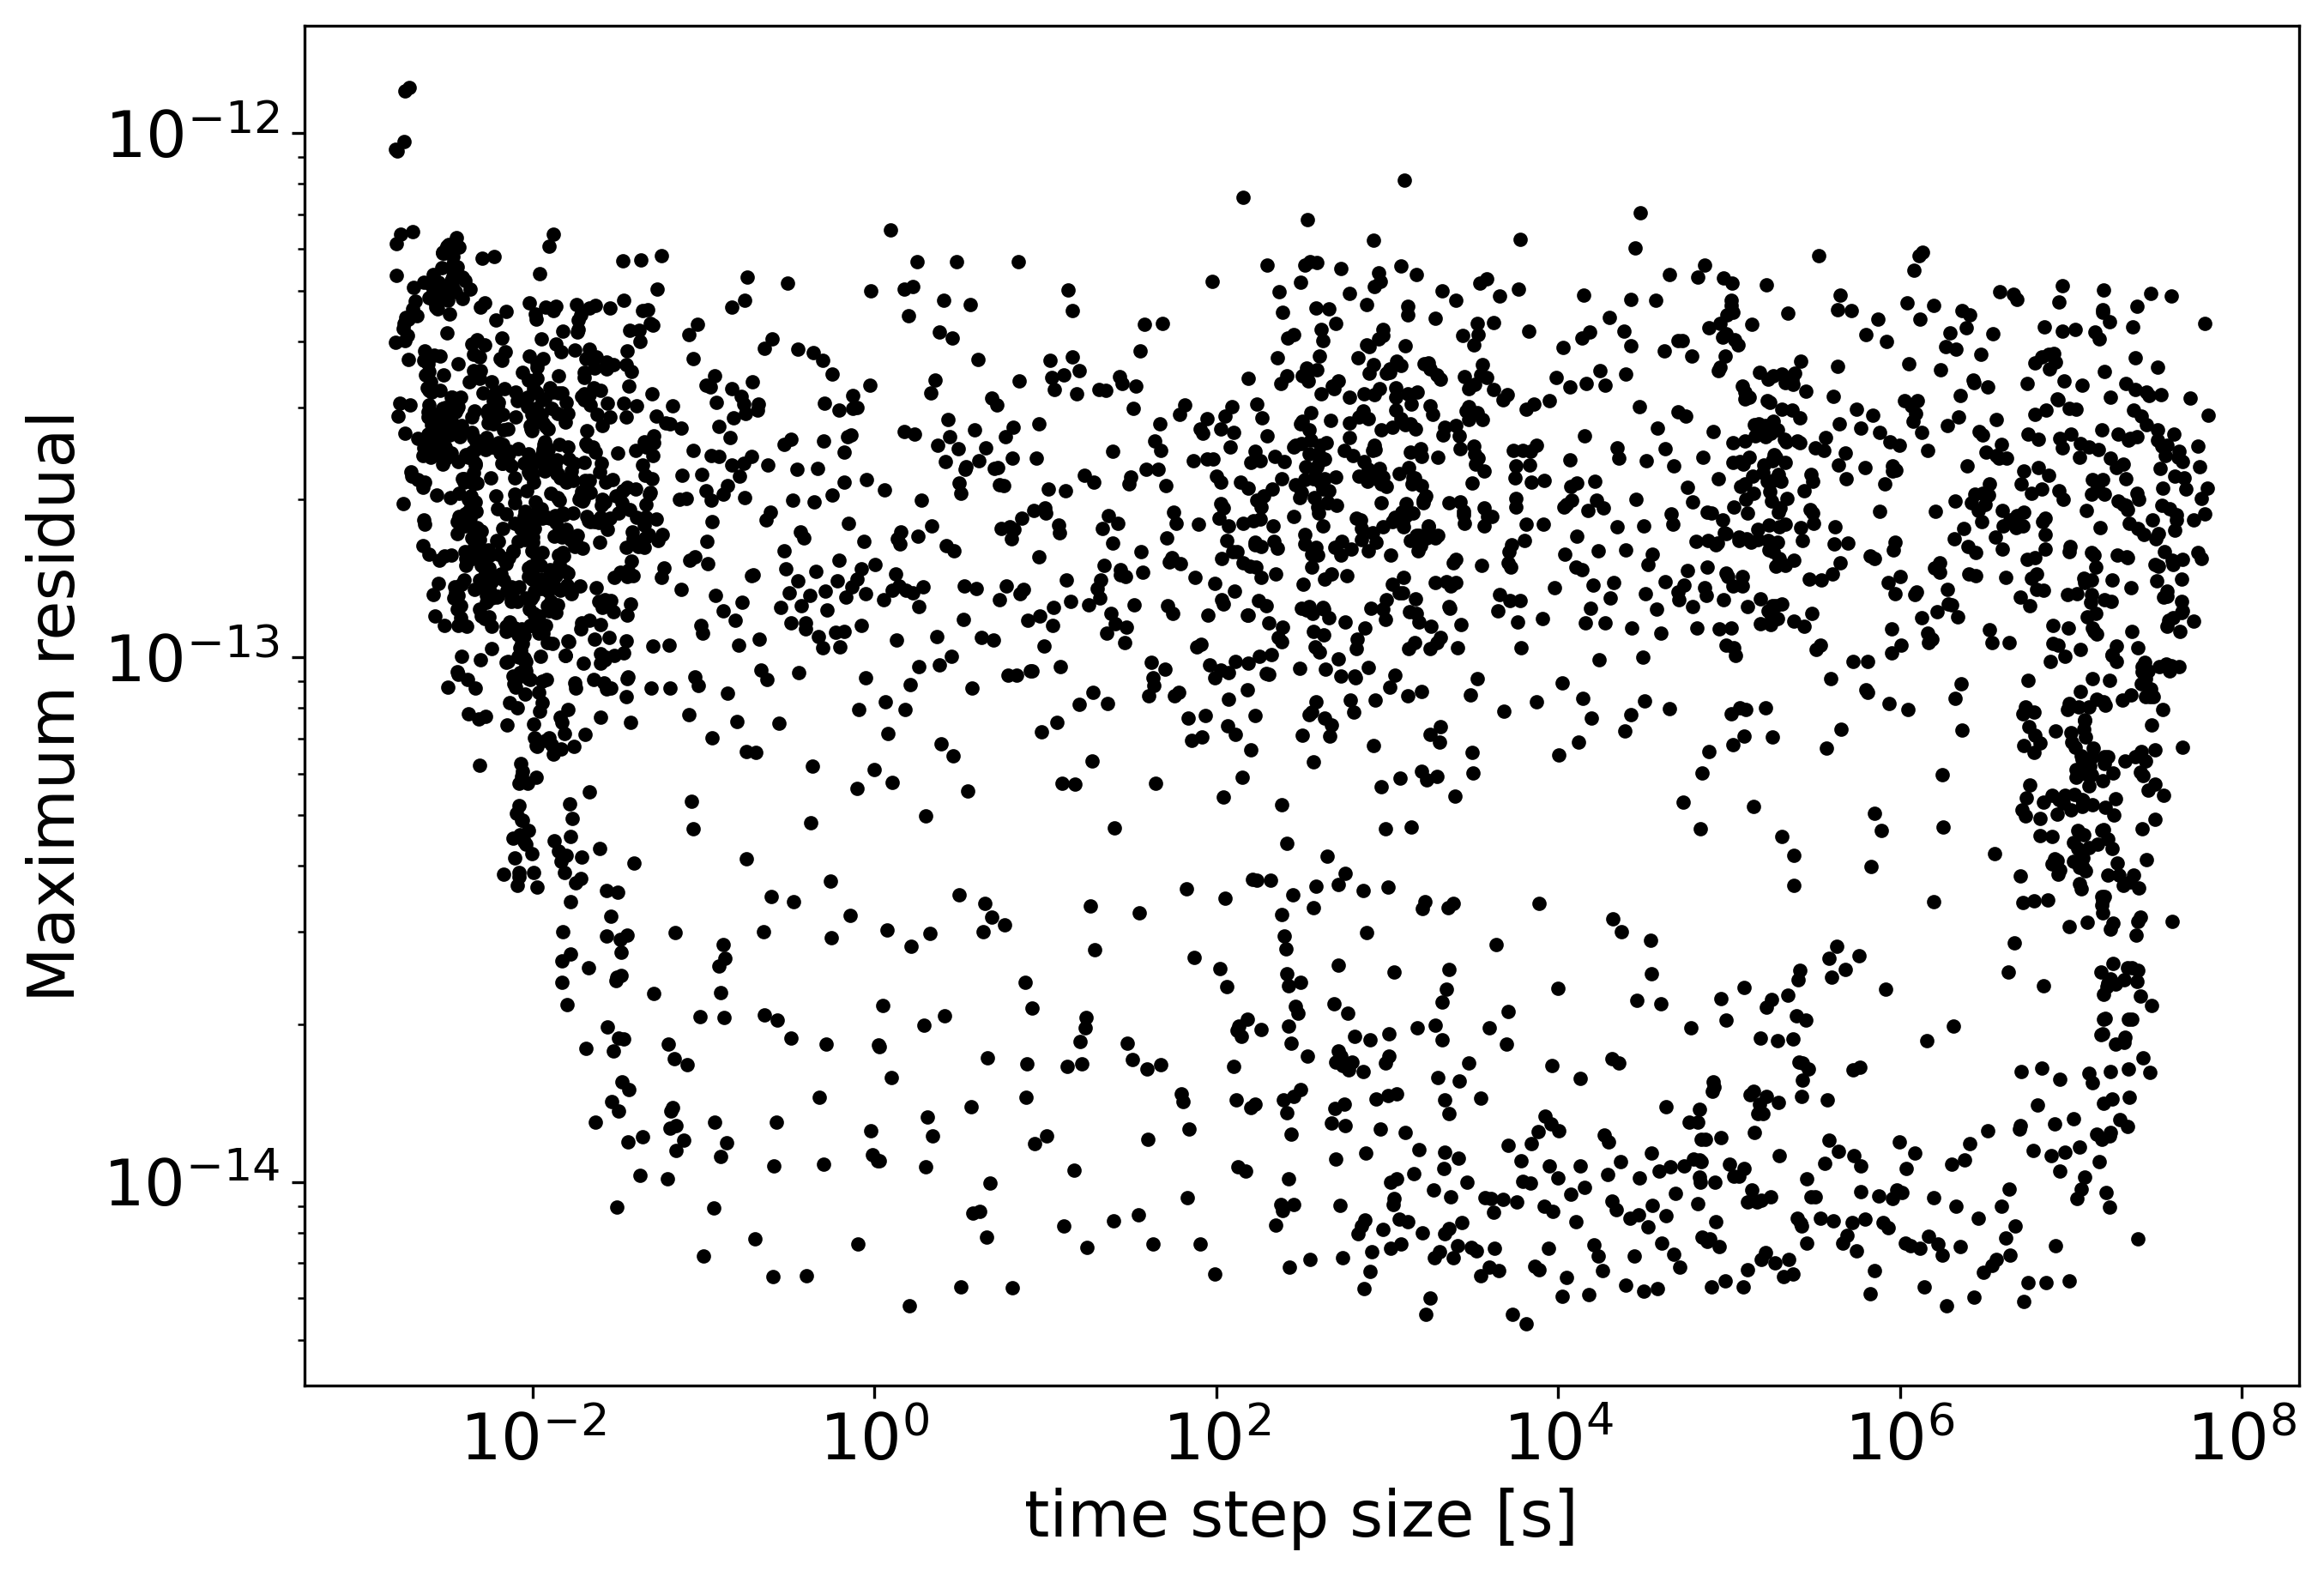
\includegraphics[width=1\textwidth]{images/TANDEMConvergenceAnalysisExtendedDAEMaxResidual_Size5.png}
		\caption{Residual of all components}
		\label{fig:convergenceIssuesExtendedDAEMaxResidual_vs_dt}
	\end{subfigure} 
	\begin{subfigure}[t]{0.45\textwidth}
		\centering
		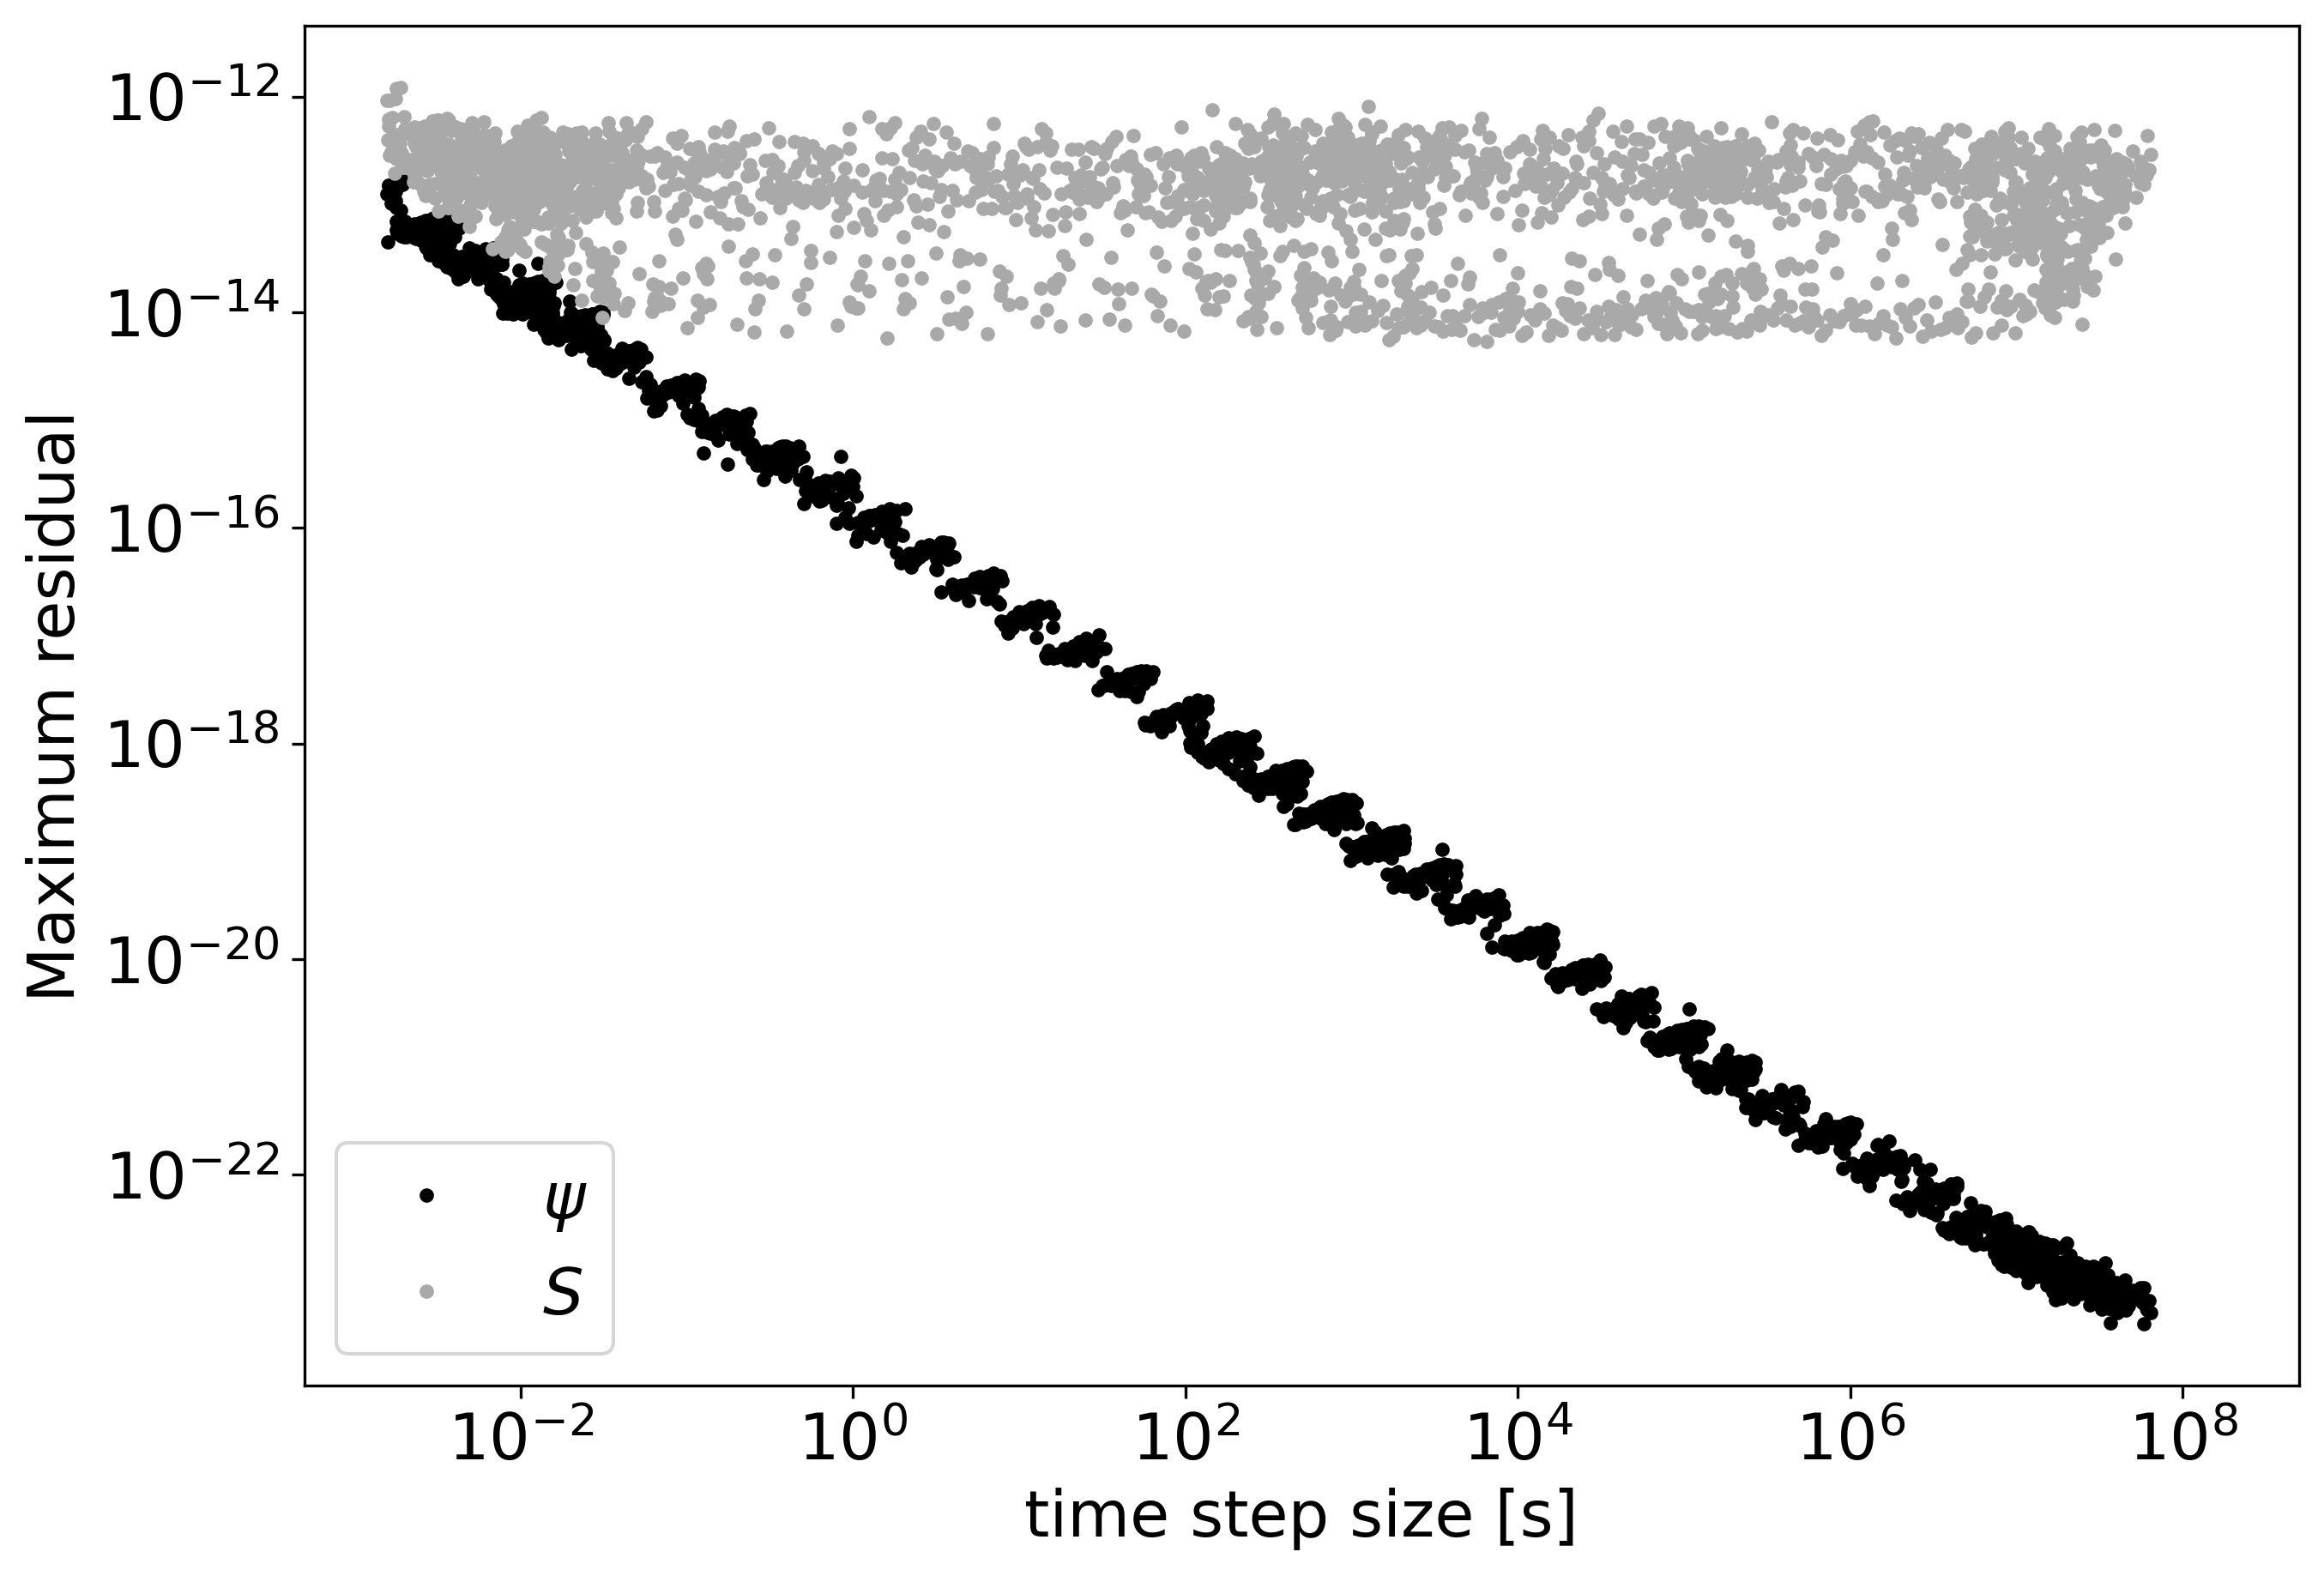
\includegraphics[width=1\textwidth]{images/TANDEMConvergenceAnalysisExtendedDAEMaxResidual_Size5_onlyPSI.png}
		\caption{Residual of the individual components $\psi$ and $S$}
		\label{fig:convergenceIssuesExtendedDAEMaxResidual_vs_dt_onlyPSI}
	\end{subfigure} 
	\caption{Minimum achievable residual norms in function of the timestep size for the extended DAE formulation with the 4th order BDF method on a small domain with 5 fault elements}
\end{figure}


In conclusion, the compact DAE formulation fails for the earthquake and can only be applied in the aseismic slip phase. Since the accuracy decreases along with the timestep size, the usual strategy to restart a step with a smaller timestep size if the nonlinear did not converge only leads to an even worse accuracy and is unsuitable.

\subsection{Stopping criterion}
\label{ssec:StoppingCriterionNewton}
The Newton iteration should be stopped when the norm of the residual becomes lower than some tolerance value or if the last Newton step could not decrease the norm further, as it happened for the compact DAE formulation. In this latter case, the Newton iteration is not rejected because the standard PETSc approach to reduce the timestep size cannot decrease the final residual error. Instead, a warning is printed to the terminal to notify the user that the Newton iteration could not reach the requested accuracy. If a $NaN$ value is encountered in the solution vector, or if the residual norm is larger than the initial norm, divergence is declared and PETSc is ordered to restart the current timestep with a smaller timestep size. \\
It makes sense to prescribe different tolerances for the components of the residual in $S$, $\psi$, $V$ or $f$ as for the time integration, since their magnitudes greatly differ. To ensure comparability with explicit methods, the friction law is always solved up to the maximum precision $\varepsilon_{max}$. The other tolerances are defined in a way that the local truncation errors in $\varepsilon^S$, $\varepsilon^\psi$ and $\varepsilon^V$ derived in \autoref{ssec:LowerBoundTimeTolerance} from $\varepsilon_{max}$ can be reached here. We use here $\varepsilon^S=4\cdot10^{-12}$, $\varepsilon^\psi=2\cdot10^{-14}$ and $\varepsilon^V=V_{min}\varepsilon_{max}/\sigma_n=2\cdot10^{-24}$. In the BDF scheme, the derivatives $\dot{x}$ are defined by the weighted sum of the component $x$ at the $k$ previous timesteps, so the error in $\dot{x}$ is driven by $C\varepsilon^x$, where the factor $C$ comes from the BDF coefficients and is minimal for large timesteps, where $C_{min}\approx10^{-7}$. The error of the functions $G$ and $H$ are approximated, as always, by a first order Taylor polynomial. Depending on the chosen formulation, the functional $\Phi$ contains a combination of the following four expressions, whose respective tolerances are limited by: 
\begin{align}
	\begin{cases}
	\Phi_S = V - \dot{S}  & (1) \\ 
	\Phi_\psi = G(\psi,V) - \dot{\psi} & (2)\\ 
	\Phi_F = F(S,\psi,V) & (3)\\ 
	\Phi_H = H(t,\psi,V) - \dot{V} & (4)
	\end{cases}
\end{align}
\begin{align}
	&\begin{cases}
	t_S < \left|C\varepsilon^S + \varepsilon^V\right| & (1)\\
	t_\psi < \left|C\varepsilon^\psi + \pdv{G}{\psi}\varepsilon^\psi + \pdv{G}{V}\varepsilon^V\right| & (2)\\
	t_F = \varepsilon_{max} & (3)\\
	t_V < \left|C\varepsilon^V + \pdv{H}{\psi}\varepsilon^\psi + \pdv{H}{V}\varepsilon^V\right| & (4)
	\end{cases} &&\Leftrightarrow&
	\begin{cases}
	t_S < 4\cdot10^{-19} & (1)\\ 
	t_\psi < 5\cdot10^{-21} & (2)\\
	t_F = 1\cdot10^{-12} & (3) \\
	t_V < 3\cdot10^{-22} & (4)
	\end{cases}
\end{align}
The 1st order ODE formulation needs the conditions (1) and (2), the extended DAE needs (1), (2) and (3), the compact DAE needs (2) and (3) and finally the second order ODE needs (1), (2) and (4). 

These values are only theoretical, and show how small the final residual norm in the Newton iteration should be to fit the time tolerances. Effectively, numerical rounding errors prevent reaching such small error values, as it has been shown for the compact DAE formulation, whose success in the earthquake is compromised for this reason. Reversely, this means that the implicit methods naturally cannot reach the same time accuracy as their explicit counterparts. By experience, the two working 1st order formulations can reach at most a final residual of $10^{-12}$ and the 2nd order ODE formulation reaches $10^{-16}$.


\subsection{Iterative solvers for the Newton step update}
In each Newton step, an expensive linear system has to be solved in $\mathcal{O}\left(n^3\right)$, which is the main bottleneck for simulations on large domains. To solve this issue, several iterative methods have been tested instead of the classical Gaussian elimination. PETSc comes along with a broad range of Krylov methods with even more preconditioners. Usable results could already be obtained with the simple Jacobi method \cite[p. 230]{IterativeSolutionMethods}. More advanced stationary iterative methods, such as Gauss-Seidel or SOR, were not used because their PETSc implementation skips the convergence test and always performs a fixed number of iterations. Further, a Krylov method has also been tested, the generalized minimal residual method (GMRES) \cite{GMRES}. In each iteration $k$, it minimizes the residual in the $k$th-Krylov subspace of the Jacobian matrix $J$ and returns the exact solution at the latest after $n$ steps, so the complexity is the same as for a direct method in the worst case. To improve its performance, both a Jacobi and a Gauss-Seidel preconditioner have been used. \\
The average number of iterations required to solve the linear system, as well as the impact of its accuracy on the Newton iteration and on the total number of timesteps are shown in Tables \ref{tab:compactODE_iterativeSolversJacobian}-\ref{tab:extendedODE_iterativeSolversJacobian} for all four formulations. The simulation length has been chosen such that exactly one earthquake happens, except for the compact DAE formulation, which generally fails to converge for small timesteps. For the ODE formulations, the iterative solver is directly applied to the Jacobian matrix as it appears in the Newton iteration and for the DAE formulations, the system is first reduced as described in \autoref{ssec:iterative_solver_Jacobian}. This is especially crucial for the extended DAE formulation since all methods fail to converge when directly applied to the Jacobian matrix. 

\subsubsection{1st order ODE formulation}
\begin{tabularx}{\textwidth}{|>{\centering\arraybackslash}m{0.3\textwidth} || c : c : c | c |}
	\hline
	& Jacobi & Jacobi-GMRES & GS-GMRES & LU \\ \hline\hline
	Average number of iterations per Newton step &  6.97  &    5.72   &    3.08  & -  \\ \hdashline
	Average number of Newton steps & 3.28  &     3.28    &   3.28  &     3.27 \\ \hdashline
	Average final Newton residual &   $1.07\cdot10^{-12}$  & $1.17\cdot10^{-12}$  & $1.33\cdot10^{-12}$  & $1.54\cdot10^{-12}$ \\ \hdashline
	Total number of timesteps & 4896  &      4906    &    4904    &    4901 \\
	\hline
	\caption{Quality of iterative solvers for the Jacobian system on a 5th-order BDF scheme with the 1st order ODE formulation on 101 fault elements for 250 years}
	\label{tab:compactODE_iterativeSolversJacobian}
\end{tabularx}

In the 1st order ODE formulation, the GMRES with a Gauss-Seidel preconditioner only needs an average of 3.08 iterations to solve the linear systems, as opposed to the Jacobi and Jacobi-GMRES methods with respectively 6.97 and 5.72 iterations. The quality of the Newton iteration and the total number of timesteps is very similar to the direct method for all three iterative methods, so the GS-GMRES method can be fully recommended for this formulation. 
\newpage 
\subsubsection{Extended DAE formulation}
\begin{tabularx}{\textwidth}{|>{\centering\arraybackslash}m{0.3\textwidth} || c : c : c | c |}
	\hline
	& Jacobi & Jacobi-GMRES & GS-GMRES & LU \\ \hline\hline
	Average number of iterations per Newton step &  7.48  &    5.11   &    2.77  & -  \\  \hdashline
	Average number of Newton steps & 4.07  &     4.82    &   4.51  &     4.23 \\  \hdashline
	Average final Newton residual &   $8.73\cdot10^{-12}$  & $1.17\cdot10^{-10}$  & $1.13\cdot10^{-10}$  & $4.53\cdot10^{-12}$ \\  \hdashline
	Total number of timesteps & 4920  &      4919    &    4919    &    4919 \\
	\hline
	\caption{Quality of iterative solvers for the Jacobian system on a 5th-order BDF scheme with the extended DAE formulation on 101 fault elements for 250 years}
	\label{tab:extendedDAE_iterativeSolversJacobian}
\end{tabularx}

In the extended DAE formulation, the three methods converge after a similar number of steps and again, the GS-GMRES method performs the best. However, both GMRES methods require slightly more Newton steps and only allow the Newton iteration to converge up to $10^{-10}$ and not $10^{-12}$ like the direct method or the Jacobi method. This reduced accuracy does not seem to impact the total number of timesteps, so the GS-GMRES can again be considered to be the best option, but there might be some simulation settings where the more accurate Jacobi method would be more appropriate.

\subsubsection{Compact DAE formulation}
\begin{tabularx}{\textwidth}{|>{\centering\arraybackslash}m{0.3\textwidth} || c : c : c | c |}
	\hline
	& Jacobi & Jacobi-GMRES & GS-GMRES & LU \\ \hline\hline
	Average number of iterations per Newton step &  10.85  &    6.58   &    3.45  & -  \\ \hdashline
	Average number of Newton steps & 3.98  &     4.01    &   3.97  &     3.97 \\ \hdashline
	Average final Newton residual &   $2.20\cdot10^{-11}$  & $2.22\cdot10^{-11}$  & $2.12\cdot10^{-11}$  & $2.04\cdot10^{-11}$ \\ \hdashline
	Total number of timesteps & 686  &      686    &    686    &    686 \\
	\hline
	\caption{Quality of iterative solvers for the Jacobian system on a 5th-order BDF scheme with the compact DAE formulation on 101 fault elements for 200 years}
	\label{tab:compactDAE_iterativeSolversJacobian}
\end{tabularx}
For the compact DAE formulation, the simulation was run only over 200 years, to avoid the earthquake for which this method does not converge. The GS-GMRES method performs again the best. Overall, more iterations are needed to converge than for its extended counterpart, albeit the comparison has only a limited significance because the latter went through an earthquake event, which is impossible for the former. 

\subsubsection{2nd order ODE formulation}
\begin{tabularx}{\textwidth}{|>{\centering\arraybackslash}m{0.3\textwidth} || c : c : c | c |}
		\hline
		& Jacobi & Jacobi-GMRES & GS-GMRES & LU \\ \hline\hline
		Average number of iterations per Newton step &  5.41  &    4.95   &    2.57  & -  \\ \hdashline
		Average number of Newton steps & 3.25  &     2.72    &   2.72  &     2.72 \\ \hdashline
		Average final Newton residual &   $1.91\cdot10^{-7}$  & $9.03\cdot10^{-16}$  & $7.85\cdot10^{-16}$  & $7.41\cdot10^{-16}$ \\ \hdashline
		Total number of timesteps & 11504  &      8308    &    8321    &    8306 \\
		 \hline
	\caption{Quality of iterative solvers for the Jacobian system on a 5th-order BDF scheme with the 2nd order ODE formulation on 101 fault elements for 250 years}
	\label{tab:extendedODE_iterativeSolversJacobian}
\end{tabularx}
Finally, in the 2nd order ODE formulation, there is a large difference between the Jacobi and the GMRES methods. The Jacobi method induces a much higher final residual in the Newton iteration, with a direct consequence on the total number of timesteps. On the other hand, with the GMRES methods, the simulation works as good as with a direct solver, and, as usual, the Gauss-Seidel preconditioner leads to fewer iterations than the Jacobi preconditioner. \\

In conclusion, iterative solvers are well-suited to update the Newton step. For all formulations, the GMRES method with a Gauss-Seidel preconditioner performs the best. The Jacobi preconditioner has the same impact on the overall performance of the simulation but requires more iterations to converge, so it does not bring any benefits. The Jacobi method has to be remembered as an alternative for the extended DAE formulation because the Newton iteration with GMRES is less accurate, which might impact the overall performance and accuracy under certain conditions. However, the Jacobi method should be avoided at any cost for the 2nd order ODE formulation, because it considerably affects the accuracy and performance of the simulation. 
	
\section{Data structure}
\label{sec:44mul4SEAS__Data}
\subsection{Block structure}
The solution vector is organized in a block structure that depends on the discretization of the DG scheme. The full 2D domain is discretized into triangular elements which each contains nodes at which the physical quantities are calculated. In our case, there are three nodes on each edge of an element, and this structure is preserved in the solution vectors and Jacobian matrices that are used in the time integration. Concretely, for one element, the values of a quantity at the three nodes are stored contiguously followed by the values of the next quantity. This structure is then repeated for all elements to form the entire solution vector. The order of the components is sketched in \autoref{fig:blockStructureScheme} for formulations that solve for the slip and the state variable. For the extended DAE and the 2nd order ODE formulations, the components of the slip rate $V_i$ are added elementwise after $\psi_i$.

\begin{figure}[H]
	\centering
	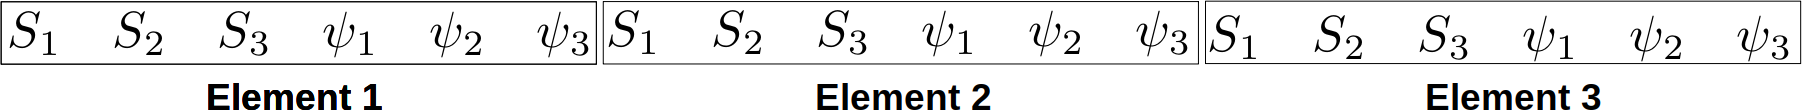
\includegraphics[width=0.9\textwidth]{images/blockStructure.png}
	\caption{Schematic representation of the components in the solution vector for the 1st order ODE and compact DAE formulations on three elements}
	\label{fig:blockStructureScheme}
\end{figure}

This block structure is also applied to the Jacobian matrices, such that they can be directly used in the Newton iteration. Setting up the matrix and the block matrix transformations in \autoref{ssec:iterative_solver_Jacobian} required thus arduous index operations.

\subsection{Memory requirements}
When the simulation will be scaled up to larger domains, memory requirements have to be taken into account. The most problematic term here will be the full matrix $\pdv{F}{S}$, whose size increases quadratically with the number of fault nodes. For example, a domain with $10^4$ fault elements and 3 nodes per fault requires, if all components are stored with double precision, 57.6GB memory just for the Jacobian matrix. Typically, such large simulations will be run on multiple cores once the code is parallelized, and the matrix is stored on multiple processors. The communication overhead to solve the Newton update will seriously hamper the performance, since there is no apparent pattern in $\pdv{F}{S}$ that could be efficiently used with parallel iterative solvers. The 1st order ODE with an explicit time integration is the only method that does not require setting up the dense matrix $\pdv{F}{S}$ and is not affected by these considerations. 

